% !TEX program = xelatex
\documentclass[final]{beamer}
\usepackage[orientation=portrait,size=a0,scale=1.2]{beamerposter}
\geometry{paperwidth=841mm,paperheight=1189mm,hmargin=25mm}
\usetheme{gemini}
\usecolortheme{inria}
\usepackage{amsmath,amssymb,graphicx,tikz,multicol,qrcode}
\usetikzlibrary{arrows.meta,calc,positioning,backgrounds,shapes.geometric}
\colorlet{inria-bleu}{inriablue}
\colorlet{inria-rouge}{inriared}
\colorlet{gris_fonce_inria}{inriagrayblue}
\colorlet{inria-2024-bleu-canard}{inriablue!80!black}
\newcommand{\PercoliaLinkedIn}{https://www.linkedin.com/company/percolia/}
\hypersetup{pdftitle={Higher-order clustering for 3D point clouds},
 pdfauthor={Louis Hauseux, Konstantin Avrachenkov, Josiane Zerubia},
 pdfsubject={AI Cluster 3IA Cote d'Azur Days 2026},colorlinks=true,urlcolor=inriablue}
\title{Higher-order clustering for 3D point clouds}
\subtitle{Exact density hierarchies and geometric tokens for 3D learning}
\author{\texorpdfstring{Louis \textsc{Hauseux}\qquad Konstantin \textsc{Avrachenkov}\qquad Josiane \textsc{Zerubia}}{Louis Hauseux, Konstantin Avrachenkov, Josiane Zerubia}}
\institute{Inria, Universit\'e C\^ote d'Azur\quad\textperiodcentered\quad NEO \& AYANA teams\quad\textperiodcentered\quad 3IA--DS4H}
\newlength{\colwidth}\setlength{\colwidth}{38.5cm}
\newcommand{\gap}{\vspace{0.7cm}}
% A visible border, not only a tinted background.
\newcommand{\formulabox}[2][inriablue]{%
  \par\vspace{0.25cm}{\centering
  \begin{tikzpicture}
    \node[draw=#1!85,fill=white,rounded corners=2mm,line width=1.2pt,
          inner xsep=5mm,inner ysep=3.5mm] {#2};
  \end{tikzpicture}\par}\vspace{0.2cm}}
\begin{document}
\begin{frame}[t]
\vspace{0.6cm}
\begin{columns}[T,onlytextwidth]
\begin{column}{\colwidth}
\begin{posterbox}{1}{Clustering}{15.8cm}
\textbf{Find groups without class labels.} Recover non-convex shapes and leave noisy points unassigned.
\vfill
\centering\resizebox{0.88\linewidth}{!}{% Generated by make_figures.py; original HDBSCAN example.
\begin{tikzpicture}[every node/.style={font=\fontsize{9}{11}\selectfont},line cap=round]
\useasboundingbox (0,-0.15) rectangle (10.3,3.5);
\begin{scope}[xshift=0.0cm]
\fill[white] (0,0) rectangle (4.4,3.0);
\draw[inriagrayblue!20,line width=.4pt] (0,0) rectangle (4.4,3.0);
\node[font=\fontsize{10}{12}\selectfont\bfseries,text=inriagrayblue] at (2.2,3.27) {Unlabelled points};
\foreach \x/\y in {0.85445/0.58016,0.92347/0.62245,0.96400/0.64097,0.73758/0.48793,0.84736/0.53076,0.85702/0.62691,0.84220/0.52770,0.98739/0.61664,0.91263/0.63038,0.93017/0.61950,0.77140/0.59607,0.90227/0.53551,2.60134/0.74684,2.90021/0.87247,2.90272/1.96239,2.84292/2.06284,2.92207/0.66751,2.83325/0.85932,2.85231/1.03819,2.90902/2.01164,2.84503/0.82704,2.84760/1.95004,2.90625/0.92256,2.89143/1.02529,2.91710/1.00464,2.86994/0.94744,2.91328/2.06049,2.90708/0.86736,2.91748/1.01671,2.90405/2.02007,2.88805/1.99971,2.86705/0.83376,3.89531/2.15368,3.94271/2.14579,3.08085/1.31233,3.08276/1.35784,3.03129/1.23991,2.93298/0.93473,3.08490/1.27301,3.92029/2.05869,3.11002/1.33100,2.94495/1.04480,2.64614/0.97353,2.03328/0.75455,2.69570/1.03244,2.70508/1.15842,2.54357/1.34849,2.73168/1.18103,2.69701/1.08995,2.69240/1.11131,2.44521/1.36327,2.81959/1.13368,3.52300/1.05858,2.10173/0.75376,3.36469/1.01287,2.10708/1.28851,2.66197/1.10947,2.53178/0.88255,2.71892/0.83788,2.40110/1.29213,2.65423/0.91287,2.89153/0.96265,2.14206/1.39696,2.57231/0.92974,2.86601/1.00483,2.51272/0.86509,2.97184/0.66974,3.05746/0.99594,2.74544/0.94715,2.54295/0.85354,3.14756/1.05527,2.33233/0.80481,2.62256/0.93038,2.73147/1.07626,2.43536/0.86582,2.72805/0.93809,2.96656/1.12749,2.77431/0.91063,2.23291/1.44365,2.81097/0.99180,2.38547/0.81553,2.14286/0.73579,3.08220/0.87184,2.22197/1.32890,2.13262/1.40719,2.52335/1.25895,2.31746/1.30002,0.66695/1.53102,0.77073/1.35949,1.91463/2.75389,0.42320/1.17697,1.54741/1.67664,0.92304/0.89898,0.52840/1.13118,1.81757/2.13447,1.71361/1.66942,0.54683/1.14723,1.14819/0.92737,0.52394/1.34272,1.14846/2.03097,0.40920/1.44074,1.76886/1.95827,1.59996/2.59798,1.25992/2.35273,1.93169/1.93089,0.62513/1.64230,1.37681/2.70017,0.67369/1.10940,1.76382/1.91852,1.70234/2.36744,1.55784/1.78861,0.61873/1.46763,1.26350/2.59596,1.82493/2.23475,0.53768/1.58137,0.87305/1.33721,0.44273/0.88496,1.90349/2.32564,1.23306/2.13444,0.47016/1.48327,1.39439/1.65093,0.96285/1.30738,1.18422/2.09495,0.72965/1.14280,1.15193/1.51863,1.13858/2.17030,1.36720/1.58086,1.16300/1.99652,1.22170/2.16951,1.54701/2.43995,1.82586/2.24062,1.26643/1.55450,1.21467/2.13784,1.02850/2.04734,1.14447/1.52157,0.63942/1.67262,1.86880/2.49869,0.40922/1.39353,0.58499/1.37281,1.19811/1.47549,1.70000/2.36784,0.76718/1.85827,1.83371/2.15107,0.73010/1.83769,0.63426/1.29535,1.83332/2.06172,1.35202/2.21242,0.99114/1.37164,1.44168/2.38797,1.60692/2.43385,0.34324/0.76353,0.54173/1.62115,1.62417/2.25350,0.49255/1.39520,1.61650/1.91900,1.61081/2.47906,1.39545/2.36295,1.28286/2.29318,1.79697/2.00823,1.80631/1.99830,0.62385/1.71638,1.25771/1.53285,1.54679/2.52513,1.70401/2.68599,1.74150/2.62710,1.31866/2.32673,1.42215/2.74968,0.76334/1.85707,0.83420/1.37776,1.58686/1.85345,0.51647/1.54590,1.42515/2.59060,1.04178/1.43683,0.47496/1.56931,1.38996/2.35469,1.51225/2.33020,2.01138/2.14037,1.78165/2.54813,0.51677/0.75342,1.77632/2.45301,1.30887/2.09114,1.71624/2.49174,0.93820/1.41268,0.80707/1.24357,1.60880/2.27124,0.72766/1.29243,1.58421/2.42210,0.79475/1.32128,0.58532/1.70185,0.98377/2.09962,1.84596/1.93044,1.37629/1.55197,0.10107/1.29621,1.33629/2.26283,0.95489/1.31512,0.34709/1.45275,1.16605/2.21974,1.30899/1.40033,0.97267/1.96566,1.78434/2.27631,0.73579/1.29519,1.25946/2.23423,0.49628/1.16295,0.40836/1.09013,0.96963/1.42979,0.67677/1.51789,1.44435/2.33804,0.43512/1.18058,0.72072/1.88853,1.33878/2.08131,1.88125/2.85000,0.85304/1.43599,0.45214/1.36395,1.59608/2.61100,1.42747/1.74472,0.61369/1.31983,1.79873/2.19516,1.40230/1.58622,1.20025/1.39840,0.58259/1.37523,0.63621/1.35170,1.10046/1.45725,1.37173/2.51852,0.67257/1.38950,0.73511/1.25110,2.03497/2.03742,1.61278/1.84942,0.92696/1.95467,0.66308/0.85685,0.72247/0.76488,1.94465/1.59189,0.75364/0.63311,0.62335/0.67675,0.66703/0.83514,2.04080/1.62827,0.63989/0.66771,0.73260/0.80865,0.68098/0.78805,2.04876/1.66918,0.73255/0.76810,2.03394/1.62954,0.67266/0.69944,1.02287/1.32752,1.88973/1.23134,0.69623/1.22965,1.77326/1.13845,2.79415/0.44551,4.03380/0.72043,3.97096/1.71020,0.17700/0.40335,0.24923/2.25996,1.32802/2.62117,0.50958/1.11385,3.62873/1.35130,0.91168/2.12314,0.73469/0.64167,3.59991/0.50605,1.48815/0.65291,1.45609/1.61003,3.67914/0.80495,2.58214/1.22399,2.66825/0.90423,1.17901/2.17285,1.87171/1.78575,2.00476/0.33569,1.27315/1.50634,2.64936/0.69383,2.17631/2.68584,0.47154/2.43306,3.40096/2.08423,1.26091/2.29618,1.68158/0.32482,4.20783/1.96668,3.34716/1.26810,2.69930/0.38571,0.25257/2.21021,3.36270/2.56778,2.21735/0.37597,0.49342/2.51785,2.24021/2.28528,3.58927/1.38670,3.44998/0.90014,3.06310/1.17358,3.96749/0.80517,0.68005/2.46460,3.77648/1.79173,0.39818/1.47476,2.56558/2.11345,2.86571/0.43609,3.16296/1.70038,3.16676/2.51178,1.41287/1.75090,4.05409/0.94505,3.55834/2.52322,3.23358/2.30832,3.86642/1.06221,3.65598/1.77975,0.18202/0.78020,1.61756/2.25801,1.52019/1.42399,2.77888/0.90779,3.42774/2.00696,2.29025/1.41256,1.49724/0.91474,4.02325/1.73209,1.68609/0.95053,2.19085/2.04675,1.46005/0.49431,2.01671/0.10000,3.04687/2.28999,1.85267/2.13700,4.14004/1.12996,2.96222/0.47015,1.36164/0.60136,0.50293/0.17173,2.77954/0.74797,4.20076/2.22503,2.95440/0.55213,3.25305/2.46351,3.90814/1.79430,2.18168/1.38651,3.07512/2.38320,2.71210/1.00750,3.13016/0.39813,0.83290/2.50738,0.52219/0.48488,4.21296/2.64514,4.05041/0.65845,0.82138/2.07884,4.28900/2.48440,2.87730/0.16711,3.90364/0.95276,1.19466/0.98602,3.06757/0.99115,3.27317/1.46485,0.59453/0.51202,2.03800/1.27318,0.26619/0.63757,2.84866/2.06351,2.76688/0.57333,0.26180/1.40779,0.53522/2.67919,4.26253/0.95546,1.51639/0.40543,2.18455/0.12977,3.44520/0.46966,0.32100/0.74472,3.76732/1.15790,4.26448/1.89427,3.69089/1.57610,4.07569/0.96030,2.39503/0.46501,1.52437/1.44946,3.42734/0.78165,3.29325/0.82213,0.37831/1.36143,3.10447/1.99790,2.06300/2.03320,4.16193/0.25208,2.67017/0.26175,1.50502/0.10924,4.30000/0.74354,3.95287/1.31892,3.13731/2.37734,3.18014/2.20855,4.22231/2.26587,1.64011/0.89682,0.29327/2.05049,1.80143/1.94854,4.03541/1.60005,0.95280/0.74213,2.13438/2.10104,1.91324/0.79253,4.21041/0.50004,3.38359/1.99581,2.10903/1.74773,3.37589/2.20517,0.25336/2.43312,2.94913/1.92170,1.84973/2.33892,3.35675/0.85979,4.00675/1.29844,0.64718/0.73238,3.56285/0.97236,2.25251/1.82064,2.25327/2.61887,2.85081/2.00852,2.53779/2.31391,0.62571/1.62949,2.47283/1.41494,2.73388/0.54351,2.03993/0.30520,3.40811/0.33500,0.24193/0.37704,4.14996/1.56086,3.08589/1.97125,0.35309/2.49690,3.82200/1.79852,2.20895/2.42842,3.94824/0.95762,1.83227/2.66156,3.63610/0.61132,2.63303/2.32410,2.22522/2.22219,3.03407/1.94477,1.59625/0.18952,1.21266/0.18480,3.21143/2.48847,0.17948/2.39468,1.02421/2.44645,3.18834/0.91609,4.18024/2.58945,3.68057/1.25849,2.96130/2.07025,0.42210/1.64393,2.98486/1.06492,2.52712/1.84107,0.64184/0.31179,0.70664/0.82340,1.04317/0.50101,0.10016/2.32052,1.45206/0.28165,2.13372/0.38994,0.31411/2.34854,3.77190/0.34818,3.08972/2.09391,1.08231/2.37010,0.40319/1.76573,1.96295/1.79038,2.34385/2.45210,4.16228/0.81741,2.42210/1.40667,0.68421/0.65803,2.58185/0.36812,2.29601/0.13939,4.02230/0.60431,2.20578/0.31993,1.05808/2.13145,2.72971/2.46266,0.97715/2.01628,1.96130/1.86240,0.61201/0.76189,4.18636/0.70220,1.45215/2.64179,2.23933/2.40912,0.57173/1.05139,2.97114/2.27276,0.35694/0.57995,0.39943/0.72691,4.04060/2.58911,1.26113/2.43142,1.68544/1.09976,0.13019/1.07363,1.82510/1.17496,2.45325/2.55970,4.08610/2.51466,1.68450/1.74142,1.68049/1.58133,4.12375/2.57497,0.28046/2.05169,2.51576/0.11765,2.99273/0.76947,2.81672/2.53210,3.96905/1.12112,0.44743/2.29242,1.72469/1.91874,3.01221/2.09327,1.56183/1.82291,4.25412/2.20109,1.43389/2.68996,0.84354/0.28159,0.40043/2.16463,3.95320/2.30300,2.79549/2.04528,1.88208/1.54669,1.37039/0.89863,0.42131/0.29050,1.20953/1.33208,0.89764/2.49873,3.41391/2.42280,3.73820/0.24280,3.44922/0.27657,4.28417/1.53188,3.66178/0.41994,3.08858/1.92093,4.23170/1.83292,0.81174/2.14710,3.23708/0.95217,2.92495/2.67123,3.15312/1.87763,3.76932/1.56541,1.48948/2.38952,3.71445/1.47875,3.13621/1.82358,3.17703/0.14509,0.53305/1.05332,3.81207/0.87259,2.41800/0.13085,4.22353/1.98353,3.00096/2.32455,2.40315/1.84816,1.96136/0.86580,3.40958/1.21080,0.14083/1.70145,0.35501/2.00440,4.28965/0.85179,3.64453/1.45873,4.20811/0.61480,0.10000/1.17732,3.29728/0.90188,3.03743/2.61188,2.43302/1.48540,2.93187/2.58792,0.16399/1.94059,3.63883/0.57243,1.04752/1.00812,3.20642/0.94890,3.28984/0.51917,3.62532/0.58791,0.50243/0.69777,0.43127/1.34538,2.20305/1.83049,1.61007/1.49831,3.53805/0.86069,0.72738/1.82576,4.28692/1.19460,3.71803/2.24198,3.20527/2.37863,1.60517/0.10600,3.35605/1.95005,1.96686/2.57246,0.66984/2.22123,4.03249/2.01001,0.10166/1.63921,3.39398/0.35216,3.86937/1.93979,3.66028/0.55309,3.53713/1.35428,3.75959/1.66423,3.97318/2.50607,2.39785/1.99634,4.13187/2.42663,2.61125/0.60536,2.49726/0.51907,0.73486/2.59695,4.26964/1.74056,0.55614/1.19169,1.70299/1.53622,3.59583/2.44827,0.78284/1.42359,4.24270/1.43783,1.18952/1.30609,3.55563/1.69243,0.47811/2.36935,3.10641/2.03978,0.72731/0.50261,1.54156/0.16936,1.89512/1.67409,0.62420/1.17861,0.81935/0.67480,0.91762/0.22929,1.30477/2.23109,0.40946/2.39246,4.10837/2.32387,2.19739/1.48098,2.11400/2.11464,3.36985/1.20497,3.14952/0.23454,3.06116/2.35112,2.26063/1.71590,3.86864/1.73043,2.99738/0.36160,2.47863/2.10106,2.70216/2.26560,3.19957/2.15691,2.09179/0.37075,3.89984/2.22154,1.40583/0.18438,3.09023/1.99132,3.92652/0.56866,4.06401/1.73651}
{\fill[inriablue!85!black,opacity=.78] (\x,\y) circle[radius=.0095];}
\foreach \x/\y in {3.42067/1.73324,3.72904/2.04721,3.56400/1.84052,3.49290/1.86797,3.34523/1.74564,3.74636/1.96418,3.48701/1.77604,3.31773/1.63041,3.68541/1.91286,3.69045/2.01368,3.68790/1.97658,3.65470/1.98723,3.53222/1.85475,3.51966/1.89023,3.25246/1.54451,3.57153/1.84252,3.84260/2.16597,3.82792/2.12409,3.42947/1.64554,3.54685/1.80258,3.15011/1.42780,3.58168/1.87557,3.46762/1.80176,3.60384/1.97074,3.43177/1.75025,3.52904/1.82721,3.55910/1.91551,3.49656/1.75295,3.66584/1.93672,3.45227/1.75363,3.74368/2.00080,3.59346/1.92927,3.10997/1.40419,3.50427/1.89099,3.69946/1.90567,3.80500/2.02682,3.64860/1.94307,3.43028/1.88970,3.40314/1.78694,3.22707/1.67120,3.37037/1.71313,3.52801/1.86390,3.66841/1.87842,3.51536/1.83681,3.35173/1.60125,3.36574/1.66755,3.44136/1.79393,3.28768/1.64360,3.37951/1.75804,3.32867/1.64468,3.44294/1.73616,3.58446/1.88078,3.38192/1.70617,3.63882/2.00386,3.41417/1.67243,3.58554/1.88341,3.55475/1.88174,3.63219/1.97460,3.49495/1.77673,3.67426/1.97878,3.29346/1.55778,3.23279/1.60266,3.79509/2.06764,3.35207/1.71062,3.67200/1.97571,3.41809/1.75447,3.11443/1.39521,3.65189/1.88805,3.48096/1.81832,3.53929/1.89408,3.53024/1.91014,3.65132/2.00795,3.60978/1.94242,3.48584/1.81001,3.54524/1.88631,3.45874/1.81445,3.35248/1.68674,3.24141/1.53599,3.31968/1.64043,3.45136/1.78944,3.39572/1.66603,3.81724/2.07384,3.37681/1.76884,3.76741/2.10300,3.72695/2.06102,3.15124/1.39853,3.53283/1.88755,3.75970/2.04674,3.32012/1.60380,3.43201/1.74393,3.60026/1.86373,3.74759/2.09431,3.59083/1.88276,3.30910/1.59205,3.11813/1.42288,3.67856/1.93374,3.72577/2.08337,3.21506/1.58384,3.34279/1.73838,3.49741/1.74953,3.14844/1.46693,3.16485/1.46717,3.39315/1.70520,3.33463/1.68078,3.51496/1.84783,3.66526/1.97687,3.15763/1.50380,3.30728/1.65000,3.16862/1.57376,3.52850/1.88784,3.40107/1.74697,3.35852/1.68555,3.75464/2.10562,3.20399/1.58193,3.31633/1.66297,3.46234/1.78082,3.63728/1.84959,3.51340/1.80533,3.48275/1.90778,3.52284/1.88662,3.32836/1.62854,3.28294/1.58947,3.75502/2.08187,3.21274/1.53489,3.59680/1.90737,3.30553/1.60746,3.68928/1.93415,3.65483/1.94231,3.66681/2.02386,3.18913/1.47055,3.73344/1.94398,3.29562/1.59633,3.56864/1.86783,3.62248/2.00366,3.71115/2.00745,3.14151/1.38896,3.75210/2.06846,3.50591/1.81148,3.12556/1.44573,3.39700/1.73257,3.80626/2.09922,3.54501/1.87678,3.41759/1.79228,3.56094/1.90727,3.43901/1.71822,3.67029/2.05858,3.64327/1.94163,3.62357/1.94112,3.40948/1.78985,3.21434/1.57802,3.36083/1.75598,3.69067/1.89192,3.74910/2.10435,3.60839/1.91020,3.86077/2.11013,3.87376/2.13383,3.20270/1.43715,3.43771/1.76841,3.83549/2.14320,3.46888/1.77490,3.79403/2.10642,3.42768/1.80037,3.19299/1.55726,3.67732/1.90633,3.49612/1.78679,3.69854/1.92718,3.48788/1.81328,3.38346/1.66696,3.56408/1.91663,3.60048/1.88818,3.61838/1.90059,3.53188/1.86856,3.23674/1.65026,3.55081/1.89537,3.61185/1.93311,3.63407/1.94606,3.66027/1.91342,3.60832/1.94143,3.31377/1.69427,3.14795/1.42528,3.41645/1.76218,3.47655/1.84519,3.60544/1.89943,3.39270/1.65602,3.73363/2.12554,3.24703/1.66158,3.74635/1.98226,3.75403/2.03078,3.10800/1.39833,3.23066/1.55536,3.66355/2.03022,3.69259/1.90478,3.49343/1.71231,3.50749/1.84104,3.46731/1.71763,3.12690/1.50780}
{\fill[inriablue!85!black,opacity=.78] (\x,\y) circle[radius=.0095];}
\foreach \x/\y in {1.19938/1.23736,0.72240/0.97124,0.90255/1.27198,1.16340/1.13400,0.75237/1.07525,0.70067/0.85671,0.89644/1.01774,0.75141/1.06061,0.87606/1.33703,0.80775/1.12690,0.87411/1.28693,0.94167/1.00795,0.82901/1.15207,1.38804/1.21815,1.66108/1.20940,1.12454/1.13400,1.00981/1.11080,1.90091/1.33851,1.73790/1.28676,0.83271/1.02272,0.73404/0.94049,1.49512/1.17182,0.76303/0.94436,1.73274/1.29117,1.11676/1.14134,1.06995/1.16058,1.00563/1.08358,1.72416/1.32649,1.90082/1.37564,0.80616/1.00041,0.77796/0.99175,1.60935/1.21813,2.05325/1.55919,1.53843/1.22355,1.69714/1.28017,0.76547/0.96593,1.95282/1.48543,0.75194/0.91851,1.29077/1.10866,1.94676/1.40690,1.97091/1.43712,1.18118/1.17234,1.82543/1.31375,2.02895/1.58491,1.93241/1.41217,0.89179/1.00170,1.93306/1.43120,0.84835/1.07390,1.24894/1.13601,0.90289/1.08437,0.85300/0.99941,1.95567/1.42810,1.69713/1.29368,0.95029/1.14167,1.17153/1.21359,1.36443/1.19063,0.79241/1.01905,1.76576/1.38759,1.39788/1.15280,1.26208/1.24849,1.86586/1.37329,1.94969/1.46740,1.54603/1.18552,0.93568/1.10023,0.79119/0.99356,1.90961/1.38701,0.78337/0.93800,1.41701/1.22242,1.98460/1.44786,1.31688/1.23790,2.00511/1.48880,1.91002/1.38800,1.81713/1.38698,1.87880/1.34353,0.90750/1.12315,1.86436/1.30237,2.07246/1.55673,1.84387/1.31385,1.85331/1.34678,1.84493/1.36255,1.16003/1.17258,1.53371/1.18471,0.86347/1.07917,1.92615/1.41137,1.36206/1.20611,1.94871/1.51319,1.06633/1.10975,0.85722/1.10267,1.81642/1.27974,1.78906/1.29776,1.48809/1.19165,0.80366/1.02791,0.71795/0.87025,1.26884/1.17145,1.07348/1.12872,1.74616/1.38103,1.00311/1.10846,1.28777/1.13255,1.79520/1.32440,1.69955/1.28016,1.92325/1.38680,1.98142/1.46426,0.73166/0.94504,1.56517/1.17127,1.95417/1.40738,1.37504/1.18571,1.93675/1.39143,0.82231/0.99798,0.79960/1.03187,1.56341/1.19925,1.44763/1.19781,1.39833/1.16675,1.01043/1.17661,0.86659/1.11654,1.90853/1.35589,0.86741/1.08526,0.84696/1.07239,1.83767/1.29060,0.75209/0.88108,2.01378/1.47907,1.73026/1.28949,0.81231/1.03220,0.90824/1.11128,0.78297/0.99097,1.78654/1.25808,2.03206/1.50763,0.81666/0.98632,1.26484/1.13113,1.94439/1.39168,1.66487/1.28250,0.79296/1.01685,1.23744/1.18415,1.71274/1.26412,1.78758/1.29404,2.05717/1.55999,1.96222/1.41419,1.25512/1.24787,0.92687/1.07242,1.65031/1.23250,1.86386/1.38788,1.46771/1.27134,1.74781/1.29882,1.46464/1.28902,1.31931/1.22341,1.50118/1.23174,1.67248/1.26853,1.59766/1.27530,0.75346/0.89050,1.96383/1.44939,1.99297/1.48887,1.05030/1.14343,1.64267/1.23734,1.28913/1.20860,1.71068/1.25377,1.22277/1.22606,1.83717/1.33260,1.64261/1.28815,0.97448/1.14244,1.89916/1.36470,1.93320/1.38991,1.35508/1.24387,1.10044/1.13579,1.38480/1.13569,0.73000/0.94407,1.70775/1.27947,1.25772/1.16073,1.24457/1.10290,0.84496/1.02892,1.40565/1.22147,0.90598/1.11775,1.24301/1.11890,1.79394/1.35667,1.79941/1.25549,1.18355/1.23706,2.03048/1.50646,0.96642/1.14794,1.29213/1.20886,1.86931/1.34683,1.87801/1.43048,1.86987/1.34170,1.95660/1.40872,1.26432/1.18834,1.60873/1.29711,1.41528/1.21449,1.24903/1.29750,0.73439/0.93135,1.31810/1.19559,1.07029/1.12245,2.02320/1.52408,1.20307/1.12527,1.78867/1.28913,0.92725/1.06428,2.00984/1.59744,1.05218/1.19870,1.98907/1.49663,1.97537/1.50588,0.81908/1.03238,0.85689/1.04975,1.09964/1.09617,1.94357/1.42750,0.83273/0.98642,1.00943/1.29002,0.93271/1.16829,0.77214/0.84402,1.00880/1.26780,0.78779/0.90356,0.79422/0.93784,1.51851/1.18392,1.42975/1.14876,1.39372/1.26782,1.38635/1.19484,1.61821/1.20336,1.64219/1.14517,1.31376/1.16474,1.19122/1.20264,1.28005/1.21203,1.06686/1.12988,1.36130/1.15039,1.10336/1.18096,1.39905/1.22230,1.48756/1.16192,1.20974/1.19124,1.65514/1.24747,1.03650/1.17273,1.38914/1.17591,1.19962/1.13848,1.27552/1.12810,1.45494/1.17039,1.30811/1.17627,1.25601/1.19088,0.99202/1.23716,1.49259/1.19761,1.29454/1.27413,1.28280/1.18582,1.39953/1.15400,1.14380/1.14658,1.46164/1.18653,0.86955/1.18196,1.36378/1.17795,1.27543/1.14404,1.53901/1.17192,0.94438/1.19523,1.15502/1.14796,0.91792/1.17244,1.49912/1.17763,1.16361/1.20016,1.02741/1.14566,1.15153/1.12503,1.22974/1.21161,1.71137/1.25833,1.43515/1.21309,1.22299/1.16312,1.62248/1.18087,1.43529/1.22739,1.65423/1.25603,1.30960/1.19042,1.14321/1.14711,1.49227/1.21046,1.06605/1.25284,1.59182/1.19113,1.22245/1.15610,1.14313/1.17131,1.41136/1.16895,1.40522/1.18790,1.26414/1.22782,1.58296/1.22458,1.49413/1.16432,1.54311/1.18096,1.34911/1.16002,1.37664/1.26852,1.63641/1.21654,1.03773/1.14272,1.65332/1.19691,1.49020/1.20863,1.19865/1.19165,1.35793/1.15717,1.46348/1.18894,1.44407/1.21870,1.73561/1.18175,0.95919/1.21605,1.24992/1.18762,1.32298/1.14386,0.97613/1.24217,1.36889/1.17376,1.28563/1.21355,1.66591/1.16061,1.35765/1.20965,1.37513/1.16120,1.09957/1.20200,1.42664/1.18057,1.08326/1.21044,1.62054/1.19297,1.06363/1.16908,1.61563/1.18329,1.06373/1.23113,1.22787/1.20267,1.29297/1.23135,1.11538/1.11733,1.21827/1.11633,1.41013/1.19789,1.47334/1.26562,1.56552/1.22073,1.33595/1.20087,1.21305/1.15007,0.94815/1.29477,2.04559/1.50509,1.66776/1.28027,0.89464/1.20410,0.74882/0.96626,0.71447/0.90066,1.75199/1.31059}
{\fill[inriablue!85!black,opacity=.78] (\x,\y) circle[radius=.0095];}
\foreach \x/\y in {1.23458/1.68018,1.32436/1.80547,1.19563/1.76373,0.90120/1.59620,1.27767/2.04711,1.26121/1.81531,0.86236/1.65687,1.48719/2.04185,1.04706/1.87268,1.21066/1.84515,1.06047/1.64308,1.10617/1.78656,1.11957/1.91967,1.31271/1.88266,0.94593/1.51885,1.34365/1.81116,1.04764/1.70900,0.68098/1.42932,1.22774/1.96023,1.30770/1.86210,1.40671/1.94970,1.46299/2.00028,1.08080/1.78363,1.33997/1.96922,0.96254/1.56458,1.20349/1.76033,1.02932/1.83978,0.81782/1.60724,1.09893/1.67232,1.51028/1.98924,1.17254/1.58091,0.67843/1.60188,0.85360/1.57894,0.88225/1.65831,0.84224/1.44702,1.15792/1.82105,1.49643/1.88760,0.76761/1.61421,1.58015/2.10872,1.28923/1.71599,0.77893/1.76066,1.63048/2.06035,0.75019/1.52309,0.71652/1.61280,1.35209/1.95454,0.78703/1.48648,1.43989/1.91765,0.87080/1.79202,1.33405/1.95904,1.60779/2.16601,1.70302/2.15604,0.98427/1.88222,1.68181/2.02899,0.93770/1.81000,0.94585/1.77169,0.75892/1.36701,1.45996/1.88808,1.09024/1.71591,1.31359/1.82220,1.14332/1.59673,1.15410/1.63159,0.93116/1.78078,1.62231/2.11435,1.49631/1.99369,0.97500/1.61303,1.50413/2.14758,1.03503/1.66374,1.51125/2.24432,1.10496/1.59727,1.26568/1.82817,1.51451/1.94277,1.48641/1.98731,1.28539/1.82531,0.78100/1.70939,0.99270/1.55427,1.59296/2.13267,1.35875/2.06605,1.30559/1.63283,0.87410/1.57689,0.84820/1.57078,1.09114/1.68490,1.20173/1.74330,1.53283/2.04842,1.41132/1.91459,0.87445/1.52762,1.66118/2.01197,1.16011/1.62440,1.46447/1.87471,1.58306/2.04237,1.58183/2.08919,0.84749/1.78765,1.47237/2.10255,1.43280/1.83529,1.39436/1.88064,1.53624/2.01924,1.24541/1.63143,1.23287/1.67668,0.89718/1.58861,1.12729/1.87409,1.40383/1.98466,0.93613/1.56562,1.51322/2.17808,1.64845/2.00761,1.07158/1.85484,1.25977/1.82109,1.43589/1.99112,1.51461/2.04466,1.55217/1.89766,1.22363/1.73626,1.05725/1.78736,1.41293/1.98563,0.91912/1.55064,1.14608/1.77532,1.02973/1.56355,0.78416/1.53683,1.38313/2.08223,1.29702/1.79973,1.54391/2.11991,1.49893/1.94387,1.02458/1.65708,1.05635/1.85902,1.10313/1.67104,0.74360/1.74115,1.29925/1.88504,1.65580/2.02868,1.69980/2.21066,1.11916/1.67001,0.84454/1.46149,0.77389/1.44562,0.95082/1.89846,1.66325/2.14804,1.25670/1.84596,1.34256/1.94907,1.34326/1.95967,1.33378/1.90414,1.09919/1.83793,0.99170/1.64386,1.33059/1.80704,0.89518/1.58706,1.48113/1.90801,1.57652/2.10000,1.37851/2.10884,0.98963/1.52857,0.75541/1.70510,0.74733/1.71534,1.53076/1.93528,0.94795/1.71518,0.79570/1.74217,1.74882/2.07337,1.00322/1.63242,1.12542/1.74095,0.94473/1.59349,1.21745/1.68380,0.71292/1.36181,1.08340/1.75607,1.17047/1.82442,1.40673/1.97699,1.51747/2.31626,0.69186/1.52468,0.90622/1.50812,1.13802/1.66961,1.39673/2.21632,1.31330/1.70518,1.09834/1.72910,1.52371/2.04488,1.49712/2.09702,0.97945/1.58591,1.18821/1.65140,1.45941/2.01083,1.36968/2.06624,1.00589/1.66395,1.49245/2.05000,0.95144/1.67545,0.81707/1.67872,1.43268/2.25411,1.05514/1.86499,1.33218/1.69484,1.54340/2.25571,1.05644/1.53002,1.07143/1.73988,1.00522/1.87826,1.42566/1.94224,1.14563/1.88027,1.48559/2.14926,0.76031/1.50331,0.72189/1.69181,1.54291/2.25204,1.73120/2.06962,1.32709/1.80375,1.36337/1.86143,1.49281/2.17984,1.69372/2.20985,1.44505/2.15601,1.41871/1.76829,1.24144/1.84948,1.16979/1.73891,1.07995/1.56621,1.38215/2.18093,1.64539/2.11405,1.13610/1.87798,1.44056/1.85702,1.73204/2.13702,1.63207/2.18183,0.82597/1.67878,0.83594/1.72243,0.87143/1.55699,0.96270/1.54233,1.34671/2.13275,1.20770/1.76710,0.72559/1.49238,0.96991/1.85095,1.21916/1.80433,1.36414/1.89241,0.91884/1.68015,0.94376/1.68178,1.15879/1.74105,1.32246/1.92930,0.84914/1.65511,1.65771/2.11792,1.43600/2.29607,0.82616/1.51675,1.04103/1.89522,0.95348/1.79322,1.35040/2.10389,0.95925/1.79524,0.66679/1.63115,1.19215/1.83515,0.99503/1.79129,0.61404/1.55261,0.95278/1.86515,1.09848/1.88690,1.28403/1.89485,1.12229/1.73758,1.13281/1.88815,1.32906/1.90715,1.49092/2.08207,0.69792/1.65426,1.19871/1.82313,1.10316/1.65652,1.50586/2.09573,1.64188/2.04861,1.03234/1.63684,1.31599/1.86835,1.49513/2.30689,1.46441/2.19041,1.77492/2.11263,1.27427/1.86713,1.43148/2.04531,1.51058/2.00308,1.59889/2.18167,1.52940/2.31276,1.31220/1.60545,0.75444/1.60560,1.56398/1.92036,1.03106/1.90896,1.54446/2.22987,0.91427/1.78799,1.77018/2.15653,1.28929/1.84663,1.71376/2.15595,1.11202/1.59765,1.32888/1.72336,1.48113/2.06141,1.53579/1.98959}
{\fill[inriablue!85!black,opacity=.78] (\x,\y) circle[radius=.0095];}
\foreach \x/\y in {1.52946/0.73763,1.14760/0.68153,2.48003/0.63280,1.36427/0.75303,1.30170/0.77941,1.87369/0.67126,1.89514/0.64099,1.70714/0.71041,1.45605/0.82760,1.77417/0.72839,1.90005/0.62639,1.58682/0.76399,2.04225/0.62439,1.75653/0.67021,1.75460/0.75487,1.29058/0.67229,1.70380/0.69570,2.12015/0.60700,1.59362/0.73757,1.26670/0.68616,1.68668/0.70159,1.79956/0.69252,1.98775/0.64774,2.23261/0.58877,1.20173/0.68694,1.70566/0.76379,2.37817/0.60124,1.90446/0.67289,1.87868/0.70487,1.64704/0.74682,2.00347/0.59749,1.49838/0.78791,1.83452/0.72985,1.61206/0.73533,1.70539/0.73258,1.31937/0.74261,1.18756/0.69358,1.74129/0.72763,1.83219/0.71399,1.68989/0.80514,1.28299/0.75515,1.05733/0.68042,1.73878/0.75150,1.26461/0.73616,1.56018/0.77601,2.04025/0.59197,1.42782/0.72086,1.55692/0.75779,1.23392/0.69989,1.64019/0.74677,1.45083/0.80232,1.17957/0.73261,1.96830/0.63143,1.76355/0.72112,1.85523/0.63804,1.24757/0.67894,1.79396/0.65769,1.44786/0.78616,1.74145/0.71554,1.45198/0.78259,1.15273/0.64702,1.50918/0.76224,1.45656/0.77659,1.76792/0.68505,1.43621/0.74104,1.22827/0.68954,1.73558/0.72018,1.71390/0.73824,1.43818/0.83175,2.11015/0.63019,1.13032/0.69752,2.15045/0.62867,1.08490/0.67280,1.27512/0.78092,2.07672/0.56664,1.83705/0.69909,1.39628/0.78788,1.88957/0.73035,1.37977/0.76459,1.50947/0.78970,1.81993/0.72268,2.03816/0.63802,1.73228/0.65452,1.26253/0.74713,1.38897/0.75607,1.26024/0.64828,1.37254/0.73978,1.76670/0.70983,1.63766/0.74566,1.78292/0.67050,1.83410/0.61865,1.85169/0.61858,1.61798/0.78211,1.59219/0.72849,1.45347/0.83756,1.79502/0.72608,1.91730/0.62861,1.86776/0.63595,1.09312/0.66972,1.78633/0.69838,2.04209/0.58486,1.44426/0.81392,1.19304/0.66661,1.38429/0.73212,1.87168/0.66681,1.31310/0.82774,1.71515/0.74397,1.77561/0.69324,1.72594/0.74350,1.26654/0.66874,1.50177/0.79374,1.52069/0.76170,1.23840/0.78217,1.49818/0.78110,1.86635/0.67521,0.98855/0.62643,1.19386/0.62689,1.34674/0.76910,2.09632/0.56384,1.21343/0.77807,2.00569/0.59385,2.39836/0.62028,1.61618/0.77965,1.42251/0.79548,1.17887/0.69068,2.09247/0.56433,1.93033/0.61950,1.92733/0.67312,1.97445/0.58913,1.55593/0.81010,1.74093/0.73508,1.77089/0.71319,1.50183/0.85284,1.52067/0.78879,1.79063/0.68302,1.66779/0.78435,1.57361/0.72053,1.72529/0.73875,1.74486/0.69763,2.04807/0.66238,1.52683/0.75101,1.10096/0.67642,1.05732/0.65624,1.67515/0.77963,1.58818/0.75810,1.31538/0.78118,1.60501/0.72132,1.72615/0.68052,2.24599/0.55116,1.37286/0.76793,1.60864/0.84658,1.67786/0.75644,1.41939/0.78180,1.08056/0.62034,1.91445/0.60640,2.08644/0.62725,1.86123/0.69249,1.42497/0.74166,1.79953/0.77270,1.82855/0.66580,1.40295/0.73189,1.79672/0.71286,1.93151/0.65078,1.79705/0.71839,1.52782/0.74506,1.48883/0.77006,1.66831/0.73387,2.11363/0.60767,2.20597/0.56693,1.60240/0.71474,1.53676/0.83180,1.72372/0.73085,1.09731/0.61931,1.45808/0.83857,1.60018/0.73884,1.51543/0.80129,2.19105/0.57982,1.40889/0.77181,1.43180/0.77534,2.15215/0.51658,1.08159/0.67917,1.40863/0.73062,1.42889/0.77826,1.65876/0.75768,1.61086/0.71946,1.37735/0.73322,1.24525/0.81428,2.01173/0.63709,1.74193/0.72086,1.69667/0.74278,1.51079/0.80877,1.38221/0.74705,1.89828/0.65952,1.32181/0.73612,1.22700/0.74580,1.98858/0.57102,1.95178/0.62234,1.74695/0.72239,1.96009/0.55879,1.23322/0.65781,1.80843/0.71169,1.90903/0.69505,1.86494/0.63015,1.25274/0.72343,1.57106/0.79063,1.23407/0.74084,1.34112/0.74123,1.08511/0.68426,1.78395/0.69292,1.33182/0.72964,1.36927/0.65667,1.36532/0.73631,2.41448/0.67037,1.58189/0.66248,1.81815/0.70701,1.60146/0.75823,1.94024/0.69250,1.34916/0.75126,1.17034/0.68987,1.70211/0.73952,1.99287/0.64704,1.47725/0.70480,1.49152/0.73327,1.29359/0.75002,1.70365/0.72139,1.49864/0.77048,1.27442/0.70970,1.33148/0.75749,1.56764/0.72195,1.65381/0.78620,1.22847/0.75249,2.17941/0.54102,2.22142/0.62152,1.19754/0.65876,1.44684/0.81788,1.30361/0.79055,1.75326/0.70230,1.29931/0.73600,1.95540/0.62341,1.98886/0.59713,1.99753/0.69429,1.96865/0.63022,1.83872/0.66184,1.92469/0.64353,1.99672/0.61071,1.99994/0.55268,1.97837/0.65452,2.02453/0.61503,1.98790/0.65424,1.97418/0.67935,1.97194/0.63241,1.92139/0.63424,1.87790/0.76896,1.90081/0.64271,1.95921/0.64449,2.01918/0.64297,1.98420/0.62150,1.95916/0.58315,1.95369/0.62333,2.00772/0.57732,1.91572/0.62168,1.88909/0.62894,2.03076/0.64339,1.98278/0.62277,2.00819/0.66053,2.00571/0.58902,1.95167/0.58955,1.92201/0.62388,1.94017/0.73966,1.93845/0.66150,1.92594/0.64465,1.95920/0.60409,1.95372/0.66681,1.93537/0.60968,1.97729/0.66528,2.03753/0.60272,1.94278/0.61352,1.98552/0.54391,1.94195/0.64567,1.91376/0.66350,1.97322/0.60595,1.96372/0.65449,2.06495/0.53911,1.86954/0.72901,1.93429/0.57972,1.89268/0.66248,1.96119/0.64990,1.97223/0.64292,2.27801/0.63108,2.33542/0.61648,2.20689/0.59185,2.13493/0.55658,2.45877/0.65127,2.17223/0.61837,2.27261/0.63329,2.19911/0.62405,2.37638/0.67989,2.41180/0.64899,2.35376/0.69066,2.24875/0.57174,2.57295/0.72526,2.38202/0.58475,2.27197/0.60487,2.51491/0.72028,2.48065/0.64071,2.17974/0.63078,2.25089/0.58445,2.36073/0.60200,2.17801/0.64428,2.24944/0.57141,2.34164/0.60878,2.24457/0.65412,2.16819/0.60720,2.38927/0.60639,2.16598/0.58462,2.37854/0.61535,2.15986/0.62374,2.33096/0.61754,2.39326/0.62472,2.47889/0.64068,2.49276/0.67279,2.23428/0.61605,2.34623/0.57875,2.24503/0.60053,2.28928/0.63412,2.25364/0.62331,2.48589/0.66890,2.36816/0.68231,2.44433/0.60883,2.24933/0.63019,2.32249/0.65105,2.57838/0.66401,2.33642/0.65425,2.21055/0.61846,2.30712/0.60896,2.40693/0.65354,2.48005/0.71202,2.41170/0.60286,2.21628/0.62248,2.40718/0.69272,2.41930/0.69261,2.31035/0.57983,2.31977/0.58532,2.38244/0.69839,2.32074/0.62492,2.20467/0.54408,2.35578/0.66274,2.25723/0.62798,2.57420/0.69379,2.38056/0.62943,2.48616/0.70637,2.39440/0.67027,2.16305/0.59785,2.38352/0.68556,2.20677/0.66020,2.22477/0.56199,2.38017/0.63593,2.40138/0.62036,2.24957/0.59328,2.49851/0.70511,2.20721/0.59967,2.44871/0.62487,2.40911/0.68527,2.43403/0.58278,2.28843/0.57127,2.36837/0.63593,2.29173/0.55105,2.17898/0.58328,2.55073/0.70741,2.55305/0.69847,2.40286/0.64483,2.49564/0.72972,2.45472/0.65108,2.37283/0.69143,2.30715/0.65675,2.22518/0.60414,2.36586/0.62938,2.32141/0.63733,2.26140/0.60710,2.25471/0.59345,2.21096/0.64472,2.33811/0.57306,2.38321/0.58578,2.23519/0.62851,2.56377/0.66429,2.34174/0.67786,2.34983/0.62816,2.28751/0.72685,2.15076/0.69612,2.16830/0.69127,1.68474/0.83385,2.60934/0.69061,1.70993/0.82129,1.31588/0.75061,2.46320/0.62864,1.50619/0.73944,1.72227/0.79176,1.59884/0.66942,1.94602/0.56631,1.64717/0.72745,2.27056/0.52346,1.69403/0.64570,1.30932/0.80065,2.03847/0.53672,2.53683/0.70284,1.66256/0.78367}
{\fill[inriablue!85!black,opacity=.78] (\x,\y) circle[radius=.0095];}
\foreach \x/\y in {2.17291/1.17705,2.31927/1.11715,2.02396/0.98164,2.20337/1.06534,2.06366/0.83978,2.36480/1.17998,2.33069/1.12156,2.05202/0.90553,2.50809/0.99765,2.46462/1.02293,2.36220/1.18648,2.15993/1.15967,2.36701/1.15185,2.07647/0.97705,2.05236/0.98479,2.13776/1.07216,2.25083/1.12669,2.10874/0.91438,2.03164/1.07307,2.52869/1.08396,2.12729/0.80033,2.41513/0.95364,2.25334/0.96711,2.41638/1.00930,2.11634/1.20203,2.13179/1.00856,2.46093/1.00666,2.10892/1.06389,2.14025/1.02769,2.38083/0.89747,2.29761/0.86722,2.27921/1.24124,2.23116/1.00132,2.07032/1.20274,2.09619/0.98937,2.14836/1.01416,2.20438/1.08497,2.06187/1.13694,2.11954/1.09173,2.03838/1.00269,2.38530/0.94845,2.26280/1.20982,2.12679/0.98281,2.15155/1.15043,2.08610/1.02188,2.20243/1.05123,2.01767/0.92566,2.49603/1.07944,2.08179/1.17669,2.09277/1.15197,2.10545/0.93893,2.45265/1.04566,2.47889/1.03404,2.19529/1.08662,2.12951/0.95048,2.40264/0.97659,2.09479/1.01986,2.09815/0.97058,2.24676/1.04922,2.19324/0.81683,2.07182/0.99517,2.28383/1.21215,2.22715/1.03306,2.07832/1.06334,2.03744/1.06914,2.33216/1.04334,2.31165/1.19896,2.18142/1.01469,2.06260/0.95964,2.61557/1.15071,2.03942/1.18307,2.27284/1.15879,2.18658/1.16177,2.60357/1.18070,2.26929/1.13829,2.11294/1.08941,2.21493/0.89533,2.31470/1.23982,2.21098/0.91194,2.28262/1.19467,2.15259/1.07124,2.13993/1.15749,2.24836/1.09226,2.40917/1.26829,2.44888/0.93693,2.32582/1.02670,2.09576/0.82591,2.37231/0.88689,2.11253/1.23495,2.09429/1.19340,2.06059/1.06315,2.03662/1.11172,2.34052/1.03454,2.09654/1.17293,2.15122/0.98950,2.18847/1.03982,2.24731/1.02338,2.37000/1.05459,2.37125/0.97102,2.26473/1.09581,2.21625/1.11616,2.43021/1.12280,2.33244/1.09159,2.33562/0.97064,2.19213/1.14839,2.06605/1.07134,2.22166/0.93040,2.05915/0.90863,2.57449/1.19170,2.22108/1.13701,2.20857/1.17715,2.17215/0.93805,2.20278/1.05289,2.09178/0.99167,2.06132/1.00859,2.17895/0.90501,2.16696/0.93188,2.22157/0.94300,2.04166/1.12654,2.37725/1.02713,2.25665/1.01077,2.26794/0.91796,2.14261/0.98380,2.07402/1.07861,2.07089/1.23912,2.47284/1.25996,2.34256/1.01261,2.42126/1.07850,2.20369/0.91533,2.12625/1.05041,2.31845/1.23345,2.08560/1.07344,2.14834/0.86605,2.50495/1.08058,2.07362/0.88284,2.12424/0.87638,2.10532/0.96117,2.09658/1.10994,2.44347/1.18257,2.06129/1.07398,2.24470/1.04387,2.09280/1.07201,2.13391/0.89534,2.32633/1.00539,2.23283/0.96159,2.38348/1.10364,2.07802/0.79446,2.25761/0.96441,2.25147/1.12490,2.15409/1.20809,2.22541/0.96621,2.28620/0.91642,2.11669/0.94799,2.30750/0.96084,2.07782/0.97513,2.27106/1.19836,2.16175/1.05794,2.23319/0.92243,2.06995/0.98783,2.25692/1.03021,2.27202/1.12061,2.10207/1.07524,2.30321/0.97122,2.21566/0.98045,2.11531/1.15756,2.27632/1.11004,2.50820/1.16042,2.44889/1.19931,2.18043/1.03159,2.23262/1.05947,2.22324/1.11330,2.08150/0.99527,2.15825/1.28959,2.34739/0.97644,2.61478/1.09869,2.08243/1.19682,2.15427/1.08187,2.27544/0.93083,2.32198/1.00238,2.13914/0.94876,2.31384/1.04525,2.17562/1.04798,2.22545/1.07799,2.25371/1.21083,2.22421/1.14787,2.16583/0.82442,2.05666/1.09930,2.37886/1.10030,2.31352/0.98093,2.29484/1.08378,2.36843/0.89395,2.21742/0.96462,2.48024/1.02555,2.19057/0.85436,2.20825/1.17351,2.11770/1.07520,2.25778/0.89980,2.26474/1.06883,2.12418/0.80586,2.32322/1.08598,2.39443/1.11668,2.28926/1.09246,2.37738/1.20175,2.22720/1.03872,2.18213/0.83448,2.54337/1.01252,2.32795/1.16088,2.19407/1.16756,2.10034/1.09008,2.17568/1.15637,2.25048/1.12659,2.15953/1.03942,2.44432/1.12395,2.16190/1.18258,2.24779/1.07291,2.17928/0.93599,2.37802/0.93591,2.29950/1.02583,2.11072/1.18788,2.44719/0.99155,2.27711/1.04319,2.12440/1.16187,2.18213/1.07275,2.17850/1.24828,2.21824/0.97600,2.18988/1.00282,2.39802/1.02728,2.07235/0.98672,2.13393/1.06187,2.39451/0.96518,2.15179/0.95115,2.20896/1.07323,2.27326/1.22271,2.11692/1.27882,2.14487/1.09531,2.30586/1.29181,2.17229/1.12570,2.22723/1.13544,2.25441/0.83247,2.46560/1.24842,2.23207/0.97889,2.21118/0.90256,2.21602/1.03528,2.58253/1.10694,2.16028/0.98444,2.12335/1.09358,2.05818/0.87559,2.30623/1.07267,2.19183/1.27707,2.22727/0.88110,2.15456/1.04105,2.28186/0.91714,2.41878/1.18756,2.26366/1.27841,2.55826/1.20782,2.26775/0.98895,2.39190/0.98757,2.07338/0.97325,2.23627/0.98681,2.15015/0.96873,2.24699/1.02478,2.39626/1.08511,2.19651/1.00454,2.19089/0.80937,2.10024/1.06802,2.42915/1.23060,2.31186/0.87460,2.44039/0.96222,2.10043/0.86752,2.10361/1.10636,2.32180/1.07493,2.20675/1.09423,2.30380/1.08836,2.12657/1.16846,2.07995/1.07480,2.20801/1.01104,2.18255/1.08303,2.11900/0.84455,2.07046/1.05973,2.54216/0.97940,2.36956/1.07423,2.17168/1.19715,2.34973/1.01448,2.25710/1.17278,2.11619/1.22003,2.48030/1.17492,2.30507/1.24545,2.25771/0.89873,2.56041/1.20622,2.15704/1.10938,2.16771/0.99625,2.19155/0.98112,2.27333/0.99822,2.20874/1.03503,2.23482/0.86933,2.37322/0.96903,2.39253/1.08250,2.01827/0.87810,2.10712/1.05074,2.27024/1.01706,2.05196/1.03170,2.22119/0.89915,2.07941/0.85508,2.36568/1.12389,2.17501/1.07967,2.44222/1.18780,2.23845/0.89259,2.12804/1.00308,2.46913/1.10181,2.16954/1.10609,2.14261/0.93085,2.41205/0.97096,2.10793/1.02641,2.08492/0.91686,2.40439/0.98274,2.03122/0.97593,2.14140/0.95071,2.53982/1.14595,2.19799/1.22581,2.39650/1.19015,2.31878/1.26269,2.24036/1.05680,2.16691/1.27885,2.03458/0.89288,2.15364/0.89985,2.08574/1.06423,2.08727/1.16685,2.40892/1.12672,2.40049/0.89165,2.10874/1.06788,2.24806/0.87896,2.50874/1.13075,2.07569/0.92203,2.31329/0.91493,2.08232/1.28019,2.31525/1.09245,2.19533/1.10976,2.30067/1.07068,2.25783/1.13740,2.31552/0.95244,2.44422/1.05960,2.17781/1.00929,2.22832/1.12485,2.07742/1.15879,2.19536/1.27641,2.55207/0.95307,2.49355/0.97854,2.01941/0.81274,2.39941/0.98066,2.25248/1.22901,2.29021/1.20590,2.40938/1.13595,2.41476/1.05888,2.40979/0.90280}
{\fill[inriablue!85!black,opacity=.78] (\x,\y) circle[radius=.0095];}
\foreach \x/\y in {2.89904/1.47845,2.85129/1.53889,2.88175/1.39096,2.88615/1.35360,2.86070/1.69583,2.88908/1.58400,2.86875/1.26218,2.88841/1.12326,2.85455/1.48344,2.83074/1.22055,2.89331/1.58384,2.83625/1.09422,2.88780/1.39194,2.90866/1.38855,2.86830/1.34402,2.91935/1.59556,2.90740/1.67698,2.86093/1.24466,2.87010/1.21881,2.86689/1.52560,2.92677/1.89621,2.88169/1.51045,2.89290/1.56976,2.85022/1.21603,2.97848/1.73347,2.91336/1.05949,2.84232/1.41955,2.90978/1.71545,2.87903/1.79915,2.89818/1.41858,2.88538/1.62532,2.84503/1.81965,2.83503/1.28948,2.94219/1.70606,2.90970/1.27156,2.86526/1.41865,2.89362/1.30768,2.84312/1.27252,2.92749/1.72051,2.90211/1.57491,2.92344/1.34382,2.92658/1.43567,2.88464/1.46224,2.89322/1.22113,2.95279/1.63474,2.85603/1.45570,2.93556/1.47077,2.91937/1.65794,2.85143/1.88266,2.85573/1.49980,2.89590/1.32561,2.86245/1.23312,2.91357/1.68388,2.81745/1.23615,2.89790/1.48574,2.89286/1.79340,2.92117/1.47508,2.89777/1.84108,2.91428/1.68425,2.94226/1.64700,2.88847/1.66057,2.92438/1.31791,2.85343/1.65934,2.95350/1.85939,2.87821/1.63600,2.90239/1.64534,2.91751/1.64606,2.90152/1.41425,2.85712/1.49648,2.90560/1.28414,2.92785/1.69774,2.89483/1.46829,2.87513/1.36849,2.94050/1.27012,2.86024/1.61820,2.88433/1.60553,2.86838/1.48799,2.89242/1.23409,2.88522/1.43583,2.88657/1.37689,2.95189/1.62711,2.88588/1.35087,2.85785/1.42575,2.90257/1.61525,2.89242/1.57042,2.84288/1.78944,2.88023/1.83355,2.87956/1.14225,2.84327/1.50142,2.87512/1.76534,2.88008/1.46237,2.85801/1.77068,2.85193/1.25593,2.92194/1.19936,2.86198/1.50812,2.87801/1.48159,2.86486/1.46026,2.93264/1.37861,2.96743/1.25530,2.88012/1.68923,2.90933/1.28721,2.90904/1.27043,2.85979/1.63340,2.92096/1.79691,2.89266/1.58252,2.88976/1.24361,2.91375/1.31600,2.92642/1.13904,2.85387/1.59956,2.92435/1.83058,2.84445/1.25282,2.86001/1.42041,2.87582/1.74336,2.90036/1.56242,2.88876/1.22457,2.89770/1.43499,2.87860/1.56912,2.88193/1.60410,2.93056/1.89244,2.89723/1.74236,2.93616/1.46918,2.87753/1.31512,2.86924/1.54113,2.93125/1.66207,2.92228/1.51822,2.89542/1.59107,2.93390/1.52689,2.91159/1.46838,2.89236/1.50595,2.88960/1.55895,2.90649/1.54443,2.86652/1.83452,2.88528/1.85897,2.90067/1.37657,2.87392/1.54044,2.90622/1.45585,2.87175/1.56564,2.92684/1.45195,2.89654/1.63454,2.90786/1.55972,2.91688/1.35341,2.89774/1.67566,2.90079/1.70505,2.91982/1.48479,2.88676/1.38604,2.84691/1.44785,2.85897/1.17267,2.89033/1.57248,2.87986/1.42938,2.84479/1.40768,2.86907/1.26994,2.89881/1.48320,2.92028/1.31604,2.85516/1.41191,2.92609/1.62706,2.84641/1.60843,2.94001/1.44992,2.92257/1.83132,2.92330/1.35235,2.90598/1.45653,2.89612/1.65410,2.95884/1.68446,2.89128/1.65410,2.89864/1.73310,2.89665/1.44203,2.91901/1.55684,2.89306/1.48195,2.96881/1.49489,2.89349/1.10383,2.89399/1.45544,2.88292/1.37384,2.90606/1.87672,2.86466/1.40526,2.87784/1.60359,2.87147/1.31341,2.93854/1.40061,2.88029/1.87663,2.98682/1.75030,2.95198/1.16213,2.88200/1.27826,2.86087/1.37245,2.93407/1.71132,2.97067/1.07782,2.94213/1.00261,2.89115/1.24762,2.86550/1.30232,2.66113/1.15290,2.89543/1.23628,2.87628/1.52978,2.78063/1.23146,2.79997/1.14522,2.86873/1.16579,2.91547/1.48019,2.97985/1.79846,2.83850/1.28893,2.80919/1.44666,2.77973/1.52402}
{\fill[inriablue!85!black,opacity=.78] (\x,\y) circle[radius=.0095];}
\end{scope}
\begin{scope}[xshift=5.9cm]
\fill[white] (0,0) rectangle (4.4,3.0);
\draw[inriagrayblue!20,line width=.4pt] (0,0) rectangle (4.4,3.0);
\node[font=\fontsize{10}{12}\selectfont\bfseries,text=inriagrayblue] at (2.2,3.27) {HDBSCAN [3]};
\foreach \x/\y in {0.85445/0.58016,0.92347/0.62245,0.96400/0.64097,0.73758/0.48793,0.84736/0.53076,0.85702/0.62691,0.84220/0.52770,0.98739/0.61664,0.91263/0.63038,0.93017/0.61950,0.77140/0.59607,0.90227/0.53551,2.60134/0.74684,2.90021/0.87247,2.90272/1.96239,2.84292/2.06284,2.92207/0.66751,2.83325/0.85932,2.85231/1.03819,2.90902/2.01164,2.84503/0.82704,2.84760/1.95004,2.90625/0.92256,2.89143/1.02529,2.91710/1.00464,2.86994/0.94744,2.91328/2.06049,2.90708/0.86736,2.91748/1.01671,2.90405/2.02007,2.88805/1.99971,2.86705/0.83376,3.89531/2.15368,3.94271/2.14579,3.08085/1.31233,3.08276/1.35784,3.03129/1.23991,2.93298/0.93473,3.08490/1.27301,3.92029/2.05869,3.11002/1.33100,2.94495/1.04480,2.64614/0.97353,2.03328/0.75455,2.69570/1.03244,2.70508/1.15842,2.54357/1.34849,2.73168/1.18103,2.69701/1.08995,2.69240/1.11131,2.44521/1.36327,2.81959/1.13368,3.52300/1.05858,2.10173/0.75376,3.36469/1.01287,2.10708/1.28851,2.66197/1.10947,2.53178/0.88255,2.71892/0.83788,2.40110/1.29213,2.65423/0.91287,2.89153/0.96265,2.14206/1.39696,2.57231/0.92974,2.86601/1.00483,2.51272/0.86509,2.97184/0.66974,3.05746/0.99594,2.74544/0.94715,2.54295/0.85354,3.14756/1.05527,2.33233/0.80481,2.62256/0.93038,2.73147/1.07626,2.43536/0.86582,2.72805/0.93809,2.96656/1.12749,2.77431/0.91063,2.23291/1.44365,2.81097/0.99180,2.38547/0.81553,2.14286/0.73579,3.08220/0.87184,2.22197/1.32890,2.13262/1.40719,2.52335/1.25895,2.31746/1.30002,0.66695/1.53102,0.77073/1.35949,1.91463/2.75389,0.42320/1.17697,1.54741/1.67664,0.92304/0.89898,0.52840/1.13118,1.81757/2.13447,1.71361/1.66942,0.54683/1.14723,1.14819/0.92737,0.52394/1.34272,1.14846/2.03097,0.40920/1.44074,1.76886/1.95827,1.59996/2.59798,1.25992/2.35273,1.93169/1.93089,0.62513/1.64230,1.37681/2.70017,0.67369/1.10940,1.76382/1.91852,1.70234/2.36744,1.55784/1.78861,0.61873/1.46763,1.26350/2.59596,1.82493/2.23475,0.53768/1.58137,0.87305/1.33721,0.44273/0.88496,1.90349/2.32564,1.23306/2.13444,0.47016/1.48327,1.39439/1.65093,0.96285/1.30738,1.18422/2.09495,0.72965/1.14280,1.15193/1.51863,1.13858/2.17030,1.36720/1.58086,1.16300/1.99652,1.22170/2.16951,1.54701/2.43995,1.82586/2.24062,1.26643/1.55450,1.21467/2.13784,1.02850/2.04734,1.14447/1.52157,0.63942/1.67262,1.86880/2.49869,0.40922/1.39353,0.58499/1.37281,1.19811/1.47549,1.70000/2.36784,0.76718/1.85827,1.83371/2.15107,0.73010/1.83769,0.63426/1.29535,1.83332/2.06172,1.35202/2.21242,0.99114/1.37164,1.44168/2.38797,1.60692/2.43385,0.34324/0.76353,0.54173/1.62115,1.62417/2.25350,0.49255/1.39520,1.61650/1.91900,1.61081/2.47906,1.39545/2.36295,1.28286/2.29318,1.79697/2.00823,1.80631/1.99830,0.62385/1.71638,1.25771/1.53285,1.54679/2.52513,1.70401/2.68599,1.74150/2.62710,1.31866/2.32673,1.42215/2.74968,0.76334/1.85707,0.83420/1.37776,1.58686/1.85345,0.51647/1.54590,1.42515/2.59060,1.04178/1.43683,0.47496/1.56931,1.38996/2.35469,1.51225/2.33020,2.01138/2.14037,1.78165/2.54813,0.51677/0.75342,1.77632/2.45301,1.30887/2.09114,1.71624/2.49174,0.93820/1.41268,0.80707/1.24357,1.60880/2.27124,0.72766/1.29243,1.58421/2.42210,0.79475/1.32128,0.58532/1.70185,0.98377/2.09962,1.84596/1.93044,1.37629/1.55197,0.10107/1.29621,1.33629/2.26283,0.95489/1.31512,0.34709/1.45275,1.16605/2.21974,1.30899/1.40033,0.97267/1.96566,1.78434/2.27631,0.73579/1.29519,1.25946/2.23423,0.49628/1.16295,0.40836/1.09013,0.96963/1.42979,0.67677/1.51789,1.44435/2.33804,0.43512/1.18058,0.72072/1.88853,1.33878/2.08131,1.88125/2.85000,0.85304/1.43599,0.45214/1.36395,1.59608/2.61100,1.42747/1.74472,0.61369/1.31983,1.79873/2.19516,1.40230/1.58622,1.20025/1.39840,0.58259/1.37523,0.63621/1.35170,1.10046/1.45725,1.37173/2.51852,0.67257/1.38950,0.73511/1.25110,2.03497/2.03742,1.61278/1.84942,0.92696/1.95467,0.66308/0.85685,0.72247/0.76488,1.94465/1.59189,0.75364/0.63311,0.62335/0.67675,0.66703/0.83514,2.04080/1.62827,0.63989/0.66771,0.73260/0.80865,0.68098/0.78805,2.04876/1.66918,0.73255/0.76810,2.03394/1.62954,0.67266/0.69944,1.02287/1.32752,1.88973/1.23134,0.69623/1.22965,1.77326/1.13845,2.79415/0.44551,4.03380/0.72043,3.97096/1.71020,0.17700/0.40335,0.24923/2.25996,1.32802/2.62117,0.50958/1.11385,3.62873/1.35130,0.91168/2.12314,0.73469/0.64167,3.59991/0.50605,1.48815/0.65291,1.45609/1.61003,3.67914/0.80495,2.58214/1.22399,2.66825/0.90423,1.17901/2.17285,1.87171/1.78575,2.00476/0.33569,1.27315/1.50634,2.64936/0.69383,2.17631/2.68584,0.47154/2.43306,3.40096/2.08423,1.26091/2.29618,1.68158/0.32482,4.20783/1.96668,3.34716/1.26810,2.69930/0.38571,0.25257/2.21021,3.36270/2.56778,2.21735/0.37597,0.49342/2.51785,2.24021/2.28528,3.58927/1.38670,3.44998/0.90014,3.06310/1.17358,3.96749/0.80517,0.68005/2.46460,3.77648/1.79173,0.39818/1.47476,2.56558/2.11345,2.86571/0.43609,3.16296/1.70038,3.16676/2.51178,1.41287/1.75090,4.05409/0.94505,3.55834/2.52322,3.23358/2.30832,3.86642/1.06221,3.65598/1.77975,0.18202/0.78020,1.61756/2.25801,1.52019/1.42399,2.77888/0.90779,3.42774/2.00696,2.29025/1.41256,1.49724/0.91474,4.02325/1.73209,1.68609/0.95053,2.19085/2.04675,1.46005/0.49431,2.01671/0.10000,3.04687/2.28999,1.85267/2.13700,4.14004/1.12996,2.96222/0.47015,1.36164/0.60136,0.50293/0.17173,2.77954/0.74797,4.20076/2.22503,2.95440/0.55213,3.25305/2.46351,3.90814/1.79430,2.18168/1.38651,3.07512/2.38320,2.71210/1.00750,3.13016/0.39813,0.83290/2.50738,0.52219/0.48488,4.21296/2.64514,4.05041/0.65845,0.82138/2.07884,4.28900/2.48440,2.87730/0.16711,3.90364/0.95276,1.19466/0.98602,3.06757/0.99115,3.27317/1.46485,0.59453/0.51202,2.03800/1.27318,0.26619/0.63757,2.84866/2.06351,2.76688/0.57333,0.26180/1.40779,0.53522/2.67919,4.26253/0.95546,1.51639/0.40543,2.18455/0.12977,3.44520/0.46966,0.32100/0.74472,3.76732/1.15790,4.26448/1.89427,3.69089/1.57610,4.07569/0.96030,2.39503/0.46501,1.52437/1.44946,3.42734/0.78165,3.29325/0.82213,0.37831/1.36143,3.10447/1.99790,2.06300/2.03320,4.16193/0.25208,2.67017/0.26175,1.50502/0.10924,4.30000/0.74354,3.95287/1.31892,3.13731/2.37734,3.18014/2.20855,4.22231/2.26587,1.64011/0.89682,0.29327/2.05049,1.80143/1.94854,4.03541/1.60005,0.95280/0.74213,2.13438/2.10104,1.91324/0.79253,4.21041/0.50004,3.38359/1.99581,2.10903/1.74773,3.37589/2.20517,0.25336/2.43312,2.94913/1.92170,1.84973/2.33892,3.35675/0.85979,4.00675/1.29844,0.64718/0.73238,3.56285/0.97236,2.25251/1.82064,2.25327/2.61887,2.85081/2.00852,2.53779/2.31391,0.62571/1.62949,2.47283/1.41494,2.73388/0.54351,2.03993/0.30520,3.40811/0.33500,0.24193/0.37704,4.14996/1.56086,3.08589/1.97125,0.35309/2.49690,3.82200/1.79852,2.20895/2.42842,3.94824/0.95762,1.83227/2.66156,3.63610/0.61132,2.63303/2.32410,2.22522/2.22219,3.03407/1.94477,1.59625/0.18952,1.21266/0.18480,3.21143/2.48847,0.17948/2.39468,1.02421/2.44645,3.18834/0.91609,4.18024/2.58945,3.68057/1.25849,2.96130/2.07025,0.42210/1.64393,2.98486/1.06492,2.52712/1.84107,0.64184/0.31179,0.70664/0.82340,1.04317/0.50101,0.10016/2.32052,1.45206/0.28165,2.13372/0.38994,0.31411/2.34854,3.77190/0.34818,3.08972/2.09391,1.08231/2.37010,0.40319/1.76573,1.96295/1.79038,2.34385/2.45210,4.16228/0.81741,2.42210/1.40667,0.68421/0.65803,2.58185/0.36812,2.29601/0.13939,4.02230/0.60431,2.20578/0.31993,1.05808/2.13145,2.72971/2.46266,0.97715/2.01628,1.96130/1.86240,0.61201/0.76189,4.18636/0.70220,1.45215/2.64179,2.23933/2.40912,0.57173/1.05139,2.97114/2.27276,0.35694/0.57995,0.39943/0.72691,4.04060/2.58911,1.26113/2.43142,1.68544/1.09976,0.13019/1.07363,1.82510/1.17496,2.45325/2.55970,4.08610/2.51466,1.68450/1.74142,1.68049/1.58133,4.12375/2.57497,0.28046/2.05169,2.51576/0.11765,2.99273/0.76947,2.81672/2.53210,3.96905/1.12112,0.44743/2.29242,1.72469/1.91874,3.01221/2.09327,1.56183/1.82291,4.25412/2.20109,1.43389/2.68996,0.84354/0.28159,0.40043/2.16463,3.95320/2.30300,2.79549/2.04528,1.88208/1.54669,1.37039/0.89863,0.42131/0.29050,1.20953/1.33208,0.89764/2.49873,3.41391/2.42280,3.73820/0.24280,3.44922/0.27657,4.28417/1.53188,3.66178/0.41994,3.08858/1.92093,4.23170/1.83292,0.81174/2.14710,3.23708/0.95217,2.92495/2.67123,3.15312/1.87763,3.76932/1.56541,1.48948/2.38952,3.71445/1.47875,3.13621/1.82358,3.17703/0.14509,0.53305/1.05332,3.81207/0.87259,2.41800/0.13085,4.22353/1.98353,3.00096/2.32455,2.40315/1.84816,1.96136/0.86580,3.40958/1.21080,0.14083/1.70145,0.35501/2.00440,4.28965/0.85179,3.64453/1.45873,4.20811/0.61480,0.10000/1.17732,3.29728/0.90188,3.03743/2.61188,2.43302/1.48540,2.93187/2.58792,0.16399/1.94059,3.63883/0.57243,1.04752/1.00812,3.20642/0.94890,3.28984/0.51917,3.62532/0.58791,0.50243/0.69777,0.43127/1.34538,2.20305/1.83049,1.61007/1.49831,3.53805/0.86069,0.72738/1.82576,4.28692/1.19460,3.71803/2.24198,3.20527/2.37863,1.60517/0.10600,3.35605/1.95005,1.96686/2.57246,0.66984/2.22123,4.03249/2.01001,0.10166/1.63921,3.39398/0.35216,3.86937/1.93979,3.66028/0.55309,3.53713/1.35428,3.75959/1.66423,3.97318/2.50607,2.39785/1.99634,4.13187/2.42663,2.61125/0.60536,2.49726/0.51907,0.73486/2.59695,4.26964/1.74056,0.55614/1.19169,1.70299/1.53622,3.59583/2.44827,0.78284/1.42359,4.24270/1.43783,1.18952/1.30609,3.55563/1.69243,0.47811/2.36935,3.10641/2.03978,0.72731/0.50261,1.54156/0.16936,1.89512/1.67409,0.62420/1.17861,0.81935/0.67480,0.91762/0.22929,1.30477/2.23109,0.40946/2.39246,4.10837/2.32387,2.19739/1.48098,2.11400/2.11464,3.36985/1.20497,3.14952/0.23454,3.06116/2.35112,2.26063/1.71590,3.86864/1.73043,2.99738/0.36160,2.47863/2.10106,2.70216/2.26560,3.19957/2.15691,2.09179/0.37075,3.89984/2.22154,1.40583/0.18438,3.09023/1.99132,3.92652/0.56866,4.06401/1.73651}
{\fill[gray!45,opacity=.78] (\x,\y) circle[radius=.0095];}
\foreach \x/\y in {3.42067/1.73324,3.72904/2.04721,3.56400/1.84052,3.49290/1.86797,3.34523/1.74564,3.74636/1.96418,3.48701/1.77604,3.31773/1.63041,3.68541/1.91286,3.69045/2.01368,3.68790/1.97658,3.65470/1.98723,3.53222/1.85475,3.51966/1.89023,3.25246/1.54451,3.57153/1.84252,3.84260/2.16597,3.82792/2.12409,3.42947/1.64554,3.54685/1.80258,3.15011/1.42780,3.58168/1.87557,3.46762/1.80176,3.60384/1.97074,3.43177/1.75025,3.52904/1.82721,3.55910/1.91551,3.49656/1.75295,3.66584/1.93672,3.45227/1.75363,3.74368/2.00080,3.59346/1.92927,3.10997/1.40419,3.50427/1.89099,3.69946/1.90567,3.80500/2.02682,3.64860/1.94307,3.43028/1.88970,3.40314/1.78694,3.22707/1.67120,3.37037/1.71313,3.52801/1.86390,3.66841/1.87842,3.51536/1.83681,3.35173/1.60125,3.36574/1.66755,3.44136/1.79393,3.28768/1.64360,3.37951/1.75804,3.32867/1.64468,3.44294/1.73616,3.58446/1.88078,3.38192/1.70617,3.63882/2.00386,3.41417/1.67243,3.58554/1.88341,3.55475/1.88174,3.63219/1.97460,3.49495/1.77673,3.67426/1.97878,3.29346/1.55778,3.23279/1.60266,3.79509/2.06764,3.35207/1.71062,3.67200/1.97571,3.41809/1.75447,3.11443/1.39521,3.65189/1.88805,3.48096/1.81832,3.53929/1.89408,3.53024/1.91014,3.65132/2.00795,3.60978/1.94242,3.48584/1.81001,3.54524/1.88631,3.45874/1.81445,3.35248/1.68674,3.24141/1.53599,3.31968/1.64043,3.45136/1.78944,3.39572/1.66603,3.81724/2.07384,3.37681/1.76884,3.76741/2.10300,3.72695/2.06102,3.15124/1.39853,3.53283/1.88755,3.75970/2.04674,3.32012/1.60380,3.43201/1.74393,3.60026/1.86373,3.74759/2.09431,3.59083/1.88276,3.30910/1.59205,3.11813/1.42288,3.67856/1.93374,3.72577/2.08337,3.21506/1.58384,3.34279/1.73838,3.49741/1.74953,3.14844/1.46693,3.16485/1.46717,3.39315/1.70520,3.33463/1.68078,3.51496/1.84783,3.66526/1.97687,3.15763/1.50380,3.30728/1.65000,3.16862/1.57376,3.52850/1.88784,3.40107/1.74697,3.35852/1.68555,3.75464/2.10562,3.20399/1.58193,3.31633/1.66297,3.46234/1.78082,3.63728/1.84959,3.51340/1.80533,3.48275/1.90778,3.52284/1.88662,3.32836/1.62854,3.28294/1.58947,3.75502/2.08187,3.21274/1.53489,3.59680/1.90737,3.30553/1.60746,3.68928/1.93415,3.65483/1.94231,3.66681/2.02386,3.18913/1.47055,3.73344/1.94398,3.29562/1.59633,3.56864/1.86783,3.62248/2.00366,3.71115/2.00745,3.14151/1.38896,3.75210/2.06846,3.50591/1.81148,3.12556/1.44573,3.39700/1.73257,3.80626/2.09922,3.54501/1.87678,3.41759/1.79228,3.56094/1.90727,3.43901/1.71822,3.67029/2.05858,3.64327/1.94163,3.62357/1.94112,3.40948/1.78985,3.21434/1.57802,3.36083/1.75598,3.69067/1.89192,3.74910/2.10435,3.60839/1.91020,3.86077/2.11013,3.87376/2.13383,3.20270/1.43715,3.43771/1.76841,3.83549/2.14320,3.46888/1.77490,3.79403/2.10642,3.42768/1.80037,3.19299/1.55726,3.67732/1.90633,3.49612/1.78679,3.69854/1.92718,3.48788/1.81328,3.38346/1.66696,3.56408/1.91663,3.60048/1.88818,3.61838/1.90059,3.53188/1.86856,3.23674/1.65026,3.55081/1.89537,3.61185/1.93311,3.63407/1.94606,3.66027/1.91342,3.60832/1.94143,3.31377/1.69427,3.14795/1.42528,3.41645/1.76218,3.47655/1.84519,3.60544/1.89943,3.39270/1.65602,3.73363/2.12554,3.24703/1.66158,3.74635/1.98226,3.75403/2.03078,3.10800/1.39833,3.23066/1.55536,3.66355/2.03022,3.69259/1.90478,3.49343/1.71231,3.50749/1.84104,3.46731/1.71763,3.12690/1.50780}
{\fill[inriablue,opacity=.78] (\x,\y) circle[radius=.0095];}
\foreach \x/\y in {1.19938/1.23736,0.72240/0.97124,0.90255/1.27198,1.16340/1.13400,0.75237/1.07525,0.70067/0.85671,0.89644/1.01774,0.75141/1.06061,0.87606/1.33703,0.80775/1.12690,0.87411/1.28693,0.94167/1.00795,0.82901/1.15207,1.38804/1.21815,1.66108/1.20940,1.12454/1.13400,1.00981/1.11080,1.90091/1.33851,1.73790/1.28676,0.83271/1.02272,0.73404/0.94049,1.49512/1.17182,0.76303/0.94436,1.73274/1.29117,1.11676/1.14134,1.06995/1.16058,1.00563/1.08358,1.72416/1.32649,1.90082/1.37564,0.80616/1.00041,0.77796/0.99175,1.60935/1.21813,2.05325/1.55919,1.53843/1.22355,1.69714/1.28017,0.76547/0.96593,1.95282/1.48543,0.75194/0.91851,1.29077/1.10866,1.94676/1.40690,1.97091/1.43712,1.18118/1.17234,1.82543/1.31375,2.02895/1.58491,1.93241/1.41217,0.89179/1.00170,1.93306/1.43120,0.84835/1.07390,1.24894/1.13601,0.90289/1.08437,0.85300/0.99941,1.95567/1.42810,1.69713/1.29368,0.95029/1.14167,1.17153/1.21359,1.36443/1.19063,0.79241/1.01905,1.76576/1.38759,1.39788/1.15280,1.26208/1.24849,1.86586/1.37329,1.94969/1.46740,1.54603/1.18552,0.93568/1.10023,0.79119/0.99356,1.90961/1.38701,0.78337/0.93800,1.41701/1.22242,1.98460/1.44786,1.31688/1.23790,2.00511/1.48880,1.91002/1.38800,1.81713/1.38698,1.87880/1.34353,0.90750/1.12315,1.86436/1.30237,2.07246/1.55673,1.84387/1.31385,1.85331/1.34678,1.84493/1.36255,1.16003/1.17258,1.53371/1.18471,0.86347/1.07917,1.92615/1.41137,1.36206/1.20611,1.94871/1.51319,1.06633/1.10975,0.85722/1.10267,1.81642/1.27974,1.78906/1.29776,1.48809/1.19165,0.80366/1.02791,0.71795/0.87025,1.26884/1.17145,1.07348/1.12872,1.74616/1.38103,1.00311/1.10846,1.28777/1.13255,1.79520/1.32440,1.69955/1.28016,1.92325/1.38680,1.98142/1.46426,0.73166/0.94504,1.56517/1.17127,1.95417/1.40738,1.37504/1.18571,1.93675/1.39143,0.82231/0.99798,0.79960/1.03187,1.56341/1.19925,1.44763/1.19781,1.39833/1.16675,1.01043/1.17661,0.86659/1.11654,1.90853/1.35589,0.86741/1.08526,0.84696/1.07239,1.83767/1.29060,0.75209/0.88108,2.01378/1.47907,1.73026/1.28949,0.81231/1.03220,0.90824/1.11128,0.78297/0.99097,1.78654/1.25808,2.03206/1.50763,0.81666/0.98632,1.26484/1.13113,1.94439/1.39168,1.66487/1.28250,0.79296/1.01685,1.23744/1.18415,1.71274/1.26412,1.78758/1.29404,2.05717/1.55999,1.96222/1.41419,1.25512/1.24787,0.92687/1.07242,1.65031/1.23250,1.86386/1.38788,1.46771/1.27134,1.74781/1.29882,1.46464/1.28902,1.31931/1.22341,1.50118/1.23174,1.67248/1.26853,1.59766/1.27530,0.75346/0.89050,1.96383/1.44939,1.99297/1.48887,1.05030/1.14343,1.64267/1.23734,1.28913/1.20860,1.71068/1.25377,1.22277/1.22606,1.83717/1.33260,1.64261/1.28815,0.97448/1.14244,1.89916/1.36470,1.93320/1.38991,1.35508/1.24387,1.10044/1.13579,1.38480/1.13569,0.73000/0.94407,1.70775/1.27947,1.25772/1.16073,1.24457/1.10290,0.84496/1.02892,1.40565/1.22147,0.90598/1.11775,1.24301/1.11890,1.79394/1.35667,1.79941/1.25549,1.18355/1.23706,2.03048/1.50646,0.96642/1.14794,1.29213/1.20886,1.86931/1.34683,1.87801/1.43048,1.86987/1.34170,1.95660/1.40872,1.26432/1.18834,1.60873/1.29711,1.41528/1.21449,1.24903/1.29750,0.73439/0.93135,1.31810/1.19559,1.07029/1.12245,2.02320/1.52408,1.20307/1.12527,1.78867/1.28913,0.92725/1.06428,2.00984/1.59744,1.05218/1.19870,1.98907/1.49663,1.97537/1.50588,0.81908/1.03238,0.85689/1.04975,1.09964/1.09617,1.94357/1.42750,0.83273/0.98642,1.00943/1.29002,0.93271/1.16829,0.77214/0.84402,1.00880/1.26780,0.78779/0.90356,0.79422/0.93784,1.51851/1.18392,1.42975/1.14876,1.39372/1.26782,1.38635/1.19484,1.61821/1.20336,1.64219/1.14517,1.31376/1.16474,1.19122/1.20264,1.28005/1.21203,1.06686/1.12988,1.36130/1.15039,1.10336/1.18096,1.39905/1.22230,1.48756/1.16192,1.20974/1.19124,1.65514/1.24747,1.03650/1.17273,1.38914/1.17591,1.19962/1.13848,1.27552/1.12810,1.45494/1.17039,1.30811/1.17627,1.25601/1.19088,0.99202/1.23716,1.49259/1.19761,1.29454/1.27413,1.28280/1.18582,1.39953/1.15400,1.14380/1.14658,1.46164/1.18653,0.86955/1.18196,1.36378/1.17795,1.27543/1.14404,1.53901/1.17192,0.94438/1.19523,1.15502/1.14796,0.91792/1.17244,1.49912/1.17763,1.16361/1.20016,1.02741/1.14566,1.15153/1.12503,1.22974/1.21161,1.71137/1.25833,1.43515/1.21309,1.22299/1.16312,1.62248/1.18087,1.43529/1.22739,1.65423/1.25603,1.30960/1.19042,1.14321/1.14711,1.49227/1.21046,1.06605/1.25284,1.59182/1.19113,1.22245/1.15610,1.14313/1.17131,1.41136/1.16895,1.40522/1.18790,1.26414/1.22782,1.58296/1.22458,1.49413/1.16432,1.54311/1.18096,1.34911/1.16002,1.37664/1.26852,1.63641/1.21654,1.03773/1.14272,1.65332/1.19691,1.49020/1.20863,1.19865/1.19165,1.35793/1.15717,1.46348/1.18894,1.44407/1.21870,1.73561/1.18175,0.95919/1.21605,1.24992/1.18762,1.32298/1.14386,0.97613/1.24217,1.36889/1.17376,1.28563/1.21355,1.66591/1.16061,1.35765/1.20965,1.37513/1.16120,1.09957/1.20200,1.42664/1.18057,1.08326/1.21044,1.62054/1.19297,1.06363/1.16908,1.61563/1.18329,1.06373/1.23113,1.22787/1.20267,1.29297/1.23135,1.11538/1.11733,1.21827/1.11633,1.41013/1.19789,1.47334/1.26562,1.56552/1.22073,1.33595/1.20087,1.21305/1.15007,0.94815/1.29477,2.04559/1.50509,1.66776/1.28027,0.89464/1.20410,0.74882/0.96626,0.71447/0.90066,1.75199/1.31059}
{\fill[inriamauve,opacity=.78] (\x,\y) circle[radius=.0095];}
\foreach \x/\y in {1.23458/1.68018,1.32436/1.80547,1.19563/1.76373,0.90120/1.59620,1.27767/2.04711,1.26121/1.81531,0.86236/1.65687,1.48719/2.04185,1.04706/1.87268,1.21066/1.84515,1.06047/1.64308,1.10617/1.78656,1.11957/1.91967,1.31271/1.88266,0.94593/1.51885,1.34365/1.81116,1.04764/1.70900,0.68098/1.42932,1.22774/1.96023,1.30770/1.86210,1.40671/1.94970,1.46299/2.00028,1.08080/1.78363,1.33997/1.96922,0.96254/1.56458,1.20349/1.76033,1.02932/1.83978,0.81782/1.60724,1.09893/1.67232,1.51028/1.98924,1.17254/1.58091,0.67843/1.60188,0.85360/1.57894,0.88225/1.65831,0.84224/1.44702,1.15792/1.82105,1.49643/1.88760,0.76761/1.61421,1.58015/2.10872,1.28923/1.71599,0.77893/1.76066,1.63048/2.06035,0.75019/1.52309,0.71652/1.61280,1.35209/1.95454,0.78703/1.48648,1.43989/1.91765,0.87080/1.79202,1.33405/1.95904,1.60779/2.16601,1.70302/2.15604,0.98427/1.88222,1.68181/2.02899,0.93770/1.81000,0.94585/1.77169,0.75892/1.36701,1.45996/1.88808,1.09024/1.71591,1.31359/1.82220,1.14332/1.59673,1.15410/1.63159,0.93116/1.78078,1.62231/2.11435,1.49631/1.99369,0.97500/1.61303,1.50413/2.14758,1.03503/1.66374,1.51125/2.24432,1.10496/1.59727,1.26568/1.82817,1.51451/1.94277,1.48641/1.98731,1.28539/1.82531,0.78100/1.70939,0.99270/1.55427,1.59296/2.13267,1.35875/2.06605,1.30559/1.63283,0.87410/1.57689,0.84820/1.57078,1.09114/1.68490,1.20173/1.74330,1.53283/2.04842,1.41132/1.91459,0.87445/1.52762,1.66118/2.01197,1.16011/1.62440,1.46447/1.87471,1.58306/2.04237,1.58183/2.08919,0.84749/1.78765,1.47237/2.10255,1.43280/1.83529,1.39436/1.88064,1.53624/2.01924,1.24541/1.63143,1.23287/1.67668,0.89718/1.58861,1.12729/1.87409,1.40383/1.98466,0.93613/1.56562,1.51322/2.17808,1.64845/2.00761,1.07158/1.85484,1.25977/1.82109,1.43589/1.99112,1.51461/2.04466,1.55217/1.89766,1.22363/1.73626,1.05725/1.78736,1.41293/1.98563,0.91912/1.55064,1.14608/1.77532,1.02973/1.56355,0.78416/1.53683,1.38313/2.08223,1.29702/1.79973,1.54391/2.11991,1.49893/1.94387,1.02458/1.65708,1.05635/1.85902,1.10313/1.67104,0.74360/1.74115,1.29925/1.88504,1.65580/2.02868,1.69980/2.21066,1.11916/1.67001,0.84454/1.46149,0.77389/1.44562,0.95082/1.89846,1.66325/2.14804,1.25670/1.84596,1.34256/1.94907,1.34326/1.95967,1.33378/1.90414,1.09919/1.83793,0.99170/1.64386,1.33059/1.80704,0.89518/1.58706,1.48113/1.90801,1.57652/2.10000,1.37851/2.10884,0.98963/1.52857,0.75541/1.70510,0.74733/1.71534,1.53076/1.93528,0.94795/1.71518,0.79570/1.74217,1.74882/2.07337,1.00322/1.63242,1.12542/1.74095,0.94473/1.59349,1.21745/1.68380,0.71292/1.36181,1.08340/1.75607,1.17047/1.82442,1.40673/1.97699,1.51747/2.31626,0.69186/1.52468,0.90622/1.50812,1.13802/1.66961,1.39673/2.21632,1.31330/1.70518,1.09834/1.72910,1.52371/2.04488,1.49712/2.09702,0.97945/1.58591,1.18821/1.65140,1.45941/2.01083,1.36968/2.06624,1.00589/1.66395,1.49245/2.05000,0.95144/1.67545,0.81707/1.67872,1.43268/2.25411,1.05514/1.86499,1.33218/1.69484,1.54340/2.25571,1.05644/1.53002,1.07143/1.73988,1.00522/1.87826,1.42566/1.94224,1.14563/1.88027,1.48559/2.14926,0.76031/1.50331,0.72189/1.69181,1.54291/2.25204,1.73120/2.06962,1.32709/1.80375,1.36337/1.86143,1.49281/2.17984,1.69372/2.20985,1.44505/2.15601,1.41871/1.76829,1.24144/1.84948,1.16979/1.73891,1.07995/1.56621,1.38215/2.18093,1.64539/2.11405,1.13610/1.87798,1.44056/1.85702,1.73204/2.13702,1.63207/2.18183,0.82597/1.67878,0.83594/1.72243,0.87143/1.55699,0.96270/1.54233,1.34671/2.13275,1.20770/1.76710,0.72559/1.49238,0.96991/1.85095,1.21916/1.80433,1.36414/1.89241,0.91884/1.68015,0.94376/1.68178,1.15879/1.74105,1.32246/1.92930,0.84914/1.65511,1.65771/2.11792,1.43600/2.29607,0.82616/1.51675,1.04103/1.89522,0.95348/1.79322,1.35040/2.10389,0.95925/1.79524,0.66679/1.63115,1.19215/1.83515,0.99503/1.79129,0.61404/1.55261,0.95278/1.86515,1.09848/1.88690,1.28403/1.89485,1.12229/1.73758,1.13281/1.88815,1.32906/1.90715,1.49092/2.08207,0.69792/1.65426,1.19871/1.82313,1.10316/1.65652,1.50586/2.09573,1.64188/2.04861,1.03234/1.63684,1.31599/1.86835,1.49513/2.30689,1.46441/2.19041,1.77492/2.11263,1.27427/1.86713,1.43148/2.04531,1.51058/2.00308,1.59889/2.18167,1.52940/2.31276,1.31220/1.60545,0.75444/1.60560,1.56398/1.92036,1.03106/1.90896,1.54446/2.22987,0.91427/1.78799,1.77018/2.15653,1.28929/1.84663,1.71376/2.15595,1.11202/1.59765,1.32888/1.72336,1.48113/2.06141,1.53579/1.98959}
{\fill[inriagreen!80!black,opacity=.78] (\x,\y) circle[radius=.0095];}
\foreach \x/\y in {1.52946/0.73763,1.14760/0.68153,2.48003/0.63280,1.36427/0.75303,1.30170/0.77941,1.87369/0.67126,1.89514/0.64099,1.70714/0.71041,1.45605/0.82760,1.77417/0.72839,1.90005/0.62639,1.58682/0.76399,2.04225/0.62439,1.75653/0.67021,1.75460/0.75487,1.29058/0.67229,1.70380/0.69570,2.12015/0.60700,1.59362/0.73757,1.26670/0.68616,1.68668/0.70159,1.79956/0.69252,1.98775/0.64774,2.23261/0.58877,1.20173/0.68694,1.70566/0.76379,2.37817/0.60124,1.90446/0.67289,1.87868/0.70487,1.64704/0.74682,2.00347/0.59749,1.49838/0.78791,1.83452/0.72985,1.61206/0.73533,1.70539/0.73258,1.31937/0.74261,1.18756/0.69358,1.74129/0.72763,1.83219/0.71399,1.68989/0.80514,1.28299/0.75515,1.05733/0.68042,1.73878/0.75150,1.26461/0.73616,1.56018/0.77601,2.04025/0.59197,1.42782/0.72086,1.55692/0.75779,1.23392/0.69989,1.64019/0.74677,1.45083/0.80232,1.17957/0.73261,1.96830/0.63143,1.76355/0.72112,1.85523/0.63804,1.24757/0.67894,1.79396/0.65769,1.44786/0.78616,1.74145/0.71554,1.45198/0.78259,1.15273/0.64702,1.50918/0.76224,1.45656/0.77659,1.76792/0.68505,1.43621/0.74104,1.22827/0.68954,1.73558/0.72018,1.71390/0.73824,1.43818/0.83175,2.11015/0.63019,1.13032/0.69752,2.15045/0.62867,1.08490/0.67280,1.27512/0.78092,2.07672/0.56664,1.83705/0.69909,1.39628/0.78788,1.88957/0.73035,1.37977/0.76459,1.50947/0.78970,1.81993/0.72268,2.03816/0.63802,1.73228/0.65452,1.26253/0.74713,1.38897/0.75607,1.26024/0.64828,1.37254/0.73978,1.76670/0.70983,1.63766/0.74566,1.78292/0.67050,1.83410/0.61865,1.85169/0.61858,1.61798/0.78211,1.59219/0.72849,1.45347/0.83756,1.79502/0.72608,1.91730/0.62861,1.86776/0.63595,1.09312/0.66972,1.78633/0.69838,2.04209/0.58486,1.44426/0.81392,1.19304/0.66661,1.38429/0.73212,1.87168/0.66681,1.31310/0.82774,1.71515/0.74397,1.77561/0.69324,1.72594/0.74350,1.26654/0.66874,1.50177/0.79374,1.52069/0.76170,1.23840/0.78217,1.49818/0.78110,1.86635/0.67521,0.98855/0.62643,1.19386/0.62689,1.34674/0.76910,2.09632/0.56384,1.21343/0.77807,2.00569/0.59385,2.39836/0.62028,1.61618/0.77965,1.42251/0.79548,1.17887/0.69068,2.09247/0.56433,1.93033/0.61950,1.92733/0.67312,1.97445/0.58913,1.55593/0.81010,1.74093/0.73508,1.77089/0.71319,1.50183/0.85284,1.52067/0.78879,1.79063/0.68302,1.66779/0.78435,1.57361/0.72053,1.72529/0.73875,1.74486/0.69763,2.04807/0.66238,1.52683/0.75101,1.10096/0.67642,1.05732/0.65624,1.67515/0.77963,1.58818/0.75810,1.31538/0.78118,1.60501/0.72132,1.72615/0.68052,2.24599/0.55116,1.37286/0.76793,1.60864/0.84658,1.67786/0.75644,1.41939/0.78180,1.08056/0.62034,1.91445/0.60640,2.08644/0.62725,1.86123/0.69249,1.42497/0.74166,1.79953/0.77270,1.82855/0.66580,1.40295/0.73189,1.79672/0.71286,1.93151/0.65078,1.79705/0.71839,1.52782/0.74506,1.48883/0.77006,1.66831/0.73387,2.11363/0.60767,2.20597/0.56693,1.60240/0.71474,1.53676/0.83180,1.72372/0.73085,1.09731/0.61931,1.45808/0.83857,1.60018/0.73884,1.51543/0.80129,2.19105/0.57982,1.40889/0.77181,1.43180/0.77534,2.15215/0.51658,1.08159/0.67917,1.40863/0.73062,1.42889/0.77826,1.65876/0.75768,1.61086/0.71946,1.37735/0.73322,1.24525/0.81428,2.01173/0.63709,1.74193/0.72086,1.69667/0.74278,1.51079/0.80877,1.38221/0.74705,1.89828/0.65952,1.32181/0.73612,1.22700/0.74580,1.98858/0.57102,1.95178/0.62234,1.74695/0.72239,1.96009/0.55879,1.23322/0.65781,1.80843/0.71169,1.90903/0.69505,1.86494/0.63015,1.25274/0.72343,1.57106/0.79063,1.23407/0.74084,1.34112/0.74123,1.08511/0.68426,1.78395/0.69292,1.33182/0.72964,1.36927/0.65667,1.36532/0.73631,2.41448/0.67037,1.58189/0.66248,1.81815/0.70701,1.60146/0.75823,1.94024/0.69250,1.34916/0.75126,1.17034/0.68987,1.70211/0.73952,1.99287/0.64704,1.47725/0.70480,1.49152/0.73327,1.29359/0.75002,1.70365/0.72139,1.49864/0.77048,1.27442/0.70970,1.33148/0.75749,1.56764/0.72195,1.65381/0.78620,1.22847/0.75249,2.17941/0.54102,2.22142/0.62152,1.19754/0.65876,1.44684/0.81788,1.30361/0.79055,1.75326/0.70230,1.29931/0.73600,1.95540/0.62341,1.98886/0.59713,1.99753/0.69429,1.96865/0.63022,1.83872/0.66184,1.92469/0.64353,1.99672/0.61071,1.99994/0.55268,1.97837/0.65452,2.02453/0.61503,1.98790/0.65424,1.97418/0.67935,1.97194/0.63241,1.92139/0.63424,1.87790/0.76896,1.90081/0.64271,1.95921/0.64449,2.01918/0.64297,1.98420/0.62150,1.95916/0.58315,1.95369/0.62333,2.00772/0.57732,1.91572/0.62168,1.88909/0.62894,2.03076/0.64339,1.98278/0.62277,2.00819/0.66053,2.00571/0.58902,1.95167/0.58955,1.92201/0.62388,1.94017/0.73966,1.93845/0.66150,1.92594/0.64465,1.95920/0.60409,1.95372/0.66681,1.93537/0.60968,1.97729/0.66528,2.03753/0.60272,1.94278/0.61352,1.98552/0.54391,1.94195/0.64567,1.91376/0.66350,1.97322/0.60595,1.96372/0.65449,2.06495/0.53911,1.86954/0.72901,1.93429/0.57972,1.89268/0.66248,1.96119/0.64990,1.97223/0.64292,2.27801/0.63108,2.33542/0.61648,2.20689/0.59185,2.13493/0.55658,2.45877/0.65127,2.17223/0.61837,2.27261/0.63329,2.19911/0.62405,2.37638/0.67989,2.41180/0.64899,2.35376/0.69066,2.24875/0.57174,2.57295/0.72526,2.38202/0.58475,2.27197/0.60487,2.51491/0.72028,2.48065/0.64071,2.17974/0.63078,2.25089/0.58445,2.36073/0.60200,2.17801/0.64428,2.24944/0.57141,2.34164/0.60878,2.24457/0.65412,2.16819/0.60720,2.38927/0.60639,2.16598/0.58462,2.37854/0.61535,2.15986/0.62374,2.33096/0.61754,2.39326/0.62472,2.47889/0.64068,2.49276/0.67279,2.23428/0.61605,2.34623/0.57875,2.24503/0.60053,2.28928/0.63412,2.25364/0.62331,2.48589/0.66890,2.36816/0.68231,2.44433/0.60883,2.24933/0.63019,2.32249/0.65105,2.57838/0.66401,2.33642/0.65425,2.21055/0.61846,2.30712/0.60896,2.40693/0.65354,2.48005/0.71202,2.41170/0.60286,2.21628/0.62248,2.40718/0.69272,2.41930/0.69261,2.31035/0.57983,2.31977/0.58532,2.38244/0.69839,2.32074/0.62492,2.20467/0.54408,2.35578/0.66274,2.25723/0.62798,2.57420/0.69379,2.38056/0.62943,2.48616/0.70637,2.39440/0.67027,2.16305/0.59785,2.38352/0.68556,2.20677/0.66020,2.22477/0.56199,2.38017/0.63593,2.40138/0.62036,2.24957/0.59328,2.49851/0.70511,2.20721/0.59967,2.44871/0.62487,2.40911/0.68527,2.43403/0.58278,2.28843/0.57127,2.36837/0.63593,2.29173/0.55105,2.17898/0.58328,2.55073/0.70741,2.55305/0.69847,2.40286/0.64483,2.49564/0.72972,2.45472/0.65108,2.37283/0.69143,2.30715/0.65675,2.22518/0.60414,2.36586/0.62938,2.32141/0.63733,2.26140/0.60710,2.25471/0.59345,2.21096/0.64472,2.33811/0.57306,2.38321/0.58578,2.23519/0.62851,2.56377/0.66429,2.34174/0.67786,2.34983/0.62816,2.28751/0.72685,2.15076/0.69612,2.16830/0.69127,1.68474/0.83385,2.60934/0.69061,1.70993/0.82129,1.31588/0.75061,2.46320/0.62864,1.50619/0.73944,1.72227/0.79176,1.59884/0.66942,1.94602/0.56631,1.64717/0.72745,2.27056/0.52346,1.69403/0.64570,1.30932/0.80065,2.03847/0.53672,2.53683/0.70284,1.66256/0.78367}
{\fill[inriared!85!black,opacity=.78] (\x,\y) circle[radius=.0095];}
\foreach \x/\y in {2.17291/1.17705,2.31927/1.11715,2.02396/0.98164,2.20337/1.06534,2.06366/0.83978,2.36480/1.17998,2.33069/1.12156,2.05202/0.90553,2.50809/0.99765,2.46462/1.02293,2.36220/1.18648,2.15993/1.15967,2.36701/1.15185,2.07647/0.97705,2.05236/0.98479,2.13776/1.07216,2.25083/1.12669,2.10874/0.91438,2.03164/1.07307,2.52869/1.08396,2.12729/0.80033,2.41513/0.95364,2.25334/0.96711,2.41638/1.00930,2.11634/1.20203,2.13179/1.00856,2.46093/1.00666,2.10892/1.06389,2.14025/1.02769,2.38083/0.89747,2.29761/0.86722,2.27921/1.24124,2.23116/1.00132,2.07032/1.20274,2.09619/0.98937,2.14836/1.01416,2.20438/1.08497,2.06187/1.13694,2.11954/1.09173,2.03838/1.00269,2.38530/0.94845,2.26280/1.20982,2.12679/0.98281,2.15155/1.15043,2.08610/1.02188,2.20243/1.05123,2.01767/0.92566,2.49603/1.07944,2.08179/1.17669,2.09277/1.15197,2.10545/0.93893,2.45265/1.04566,2.47889/1.03404,2.19529/1.08662,2.12951/0.95048,2.40264/0.97659,2.09479/1.01986,2.09815/0.97058,2.24676/1.04922,2.19324/0.81683,2.07182/0.99517,2.28383/1.21215,2.22715/1.03306,2.07832/1.06334,2.03744/1.06914,2.33216/1.04334,2.31165/1.19896,2.18142/1.01469,2.06260/0.95964,2.61557/1.15071,2.03942/1.18307,2.27284/1.15879,2.18658/1.16177,2.60357/1.18070,2.26929/1.13829,2.11294/1.08941,2.21493/0.89533,2.31470/1.23982,2.21098/0.91194,2.28262/1.19467,2.15259/1.07124,2.13993/1.15749,2.24836/1.09226,2.40917/1.26829,2.44888/0.93693,2.32582/1.02670,2.09576/0.82591,2.37231/0.88689,2.11253/1.23495,2.09429/1.19340,2.06059/1.06315,2.03662/1.11172,2.34052/1.03454,2.09654/1.17293,2.15122/0.98950,2.18847/1.03982,2.24731/1.02338,2.37000/1.05459,2.37125/0.97102,2.26473/1.09581,2.21625/1.11616,2.43021/1.12280,2.33244/1.09159,2.33562/0.97064,2.19213/1.14839,2.06605/1.07134,2.22166/0.93040,2.05915/0.90863,2.57449/1.19170,2.22108/1.13701,2.20857/1.17715,2.17215/0.93805,2.20278/1.05289,2.09178/0.99167,2.06132/1.00859,2.17895/0.90501,2.16696/0.93188,2.22157/0.94300,2.04166/1.12654,2.37725/1.02713,2.25665/1.01077,2.26794/0.91796,2.14261/0.98380,2.07402/1.07861,2.07089/1.23912,2.47284/1.25996,2.34256/1.01261,2.42126/1.07850,2.20369/0.91533,2.12625/1.05041,2.31845/1.23345,2.08560/1.07344,2.14834/0.86605,2.50495/1.08058,2.07362/0.88284,2.12424/0.87638,2.10532/0.96117,2.09658/1.10994,2.44347/1.18257,2.06129/1.07398,2.24470/1.04387,2.09280/1.07201,2.13391/0.89534,2.32633/1.00539,2.23283/0.96159,2.38348/1.10364,2.07802/0.79446,2.25761/0.96441,2.25147/1.12490,2.15409/1.20809,2.22541/0.96621,2.28620/0.91642,2.11669/0.94799,2.30750/0.96084,2.07782/0.97513,2.27106/1.19836,2.16175/1.05794,2.23319/0.92243,2.06995/0.98783,2.25692/1.03021,2.27202/1.12061,2.10207/1.07524,2.30321/0.97122,2.21566/0.98045,2.11531/1.15756,2.27632/1.11004,2.50820/1.16042,2.44889/1.19931,2.18043/1.03159,2.23262/1.05947,2.22324/1.11330,2.08150/0.99527,2.15825/1.28959,2.34739/0.97644,2.61478/1.09869,2.08243/1.19682,2.15427/1.08187,2.27544/0.93083,2.32198/1.00238,2.13914/0.94876,2.31384/1.04525,2.17562/1.04798,2.22545/1.07799,2.25371/1.21083,2.22421/1.14787,2.16583/0.82442,2.05666/1.09930,2.37886/1.10030,2.31352/0.98093,2.29484/1.08378,2.36843/0.89395,2.21742/0.96462,2.48024/1.02555,2.19057/0.85436,2.20825/1.17351,2.11770/1.07520,2.25778/0.89980,2.26474/1.06883,2.12418/0.80586,2.32322/1.08598,2.39443/1.11668,2.28926/1.09246,2.37738/1.20175,2.22720/1.03872,2.18213/0.83448,2.54337/1.01252,2.32795/1.16088,2.19407/1.16756,2.10034/1.09008,2.17568/1.15637,2.25048/1.12659,2.15953/1.03942,2.44432/1.12395,2.16190/1.18258,2.24779/1.07291,2.17928/0.93599,2.37802/0.93591,2.29950/1.02583,2.11072/1.18788,2.44719/0.99155,2.27711/1.04319,2.12440/1.16187,2.18213/1.07275,2.17850/1.24828,2.21824/0.97600,2.18988/1.00282,2.39802/1.02728,2.07235/0.98672,2.13393/1.06187,2.39451/0.96518,2.15179/0.95115,2.20896/1.07323,2.27326/1.22271,2.11692/1.27882,2.14487/1.09531,2.30586/1.29181,2.17229/1.12570,2.22723/1.13544,2.25441/0.83247,2.46560/1.24842,2.23207/0.97889,2.21118/0.90256,2.21602/1.03528,2.58253/1.10694,2.16028/0.98444,2.12335/1.09358,2.05818/0.87559,2.30623/1.07267,2.19183/1.27707,2.22727/0.88110,2.15456/1.04105,2.28186/0.91714,2.41878/1.18756,2.26366/1.27841,2.55826/1.20782,2.26775/0.98895,2.39190/0.98757,2.07338/0.97325,2.23627/0.98681,2.15015/0.96873,2.24699/1.02478,2.39626/1.08511,2.19651/1.00454,2.19089/0.80937,2.10024/1.06802,2.42915/1.23060,2.31186/0.87460,2.44039/0.96222,2.10043/0.86752,2.10361/1.10636,2.32180/1.07493,2.20675/1.09423,2.30380/1.08836,2.12657/1.16846,2.07995/1.07480,2.20801/1.01104,2.18255/1.08303,2.11900/0.84455,2.07046/1.05973,2.54216/0.97940,2.36956/1.07423,2.17168/1.19715,2.34973/1.01448,2.25710/1.17278,2.11619/1.22003,2.48030/1.17492,2.30507/1.24545,2.25771/0.89873,2.56041/1.20622,2.15704/1.10938,2.16771/0.99625,2.19155/0.98112,2.27333/0.99822,2.20874/1.03503,2.23482/0.86933,2.37322/0.96903,2.39253/1.08250,2.01827/0.87810,2.10712/1.05074,2.27024/1.01706,2.05196/1.03170,2.22119/0.89915,2.07941/0.85508,2.36568/1.12389,2.17501/1.07967,2.44222/1.18780,2.23845/0.89259,2.12804/1.00308,2.46913/1.10181,2.16954/1.10609,2.14261/0.93085,2.41205/0.97096,2.10793/1.02641,2.08492/0.91686,2.40439/0.98274,2.03122/0.97593,2.14140/0.95071,2.53982/1.14595,2.19799/1.22581,2.39650/1.19015,2.31878/1.26269,2.24036/1.05680,2.16691/1.27885,2.03458/0.89288,2.15364/0.89985,2.08574/1.06423,2.08727/1.16685,2.40892/1.12672,2.40049/0.89165,2.10874/1.06788,2.24806/0.87896,2.50874/1.13075,2.07569/0.92203,2.31329/0.91493,2.08232/1.28019,2.31525/1.09245,2.19533/1.10976,2.30067/1.07068,2.25783/1.13740,2.31552/0.95244,2.44422/1.05960,2.17781/1.00929,2.22832/1.12485,2.07742/1.15879,2.19536/1.27641,2.55207/0.95307,2.49355/0.97854,2.01941/0.81274,2.39941/0.98066,2.25248/1.22901,2.29021/1.20590,2.40938/1.13595,2.41476/1.05888,2.40979/0.90280}
{\fill[inrialightblue!80!black,opacity=.78] (\x,\y) circle[radius=.0095];}
\foreach \x/\y in {2.89904/1.47845,2.85129/1.53889,2.88175/1.39096,2.88615/1.35360,2.86070/1.69583,2.88908/1.58400,2.86875/1.26218,2.88841/1.12326,2.85455/1.48344,2.83074/1.22055,2.89331/1.58384,2.83625/1.09422,2.88780/1.39194,2.90866/1.38855,2.86830/1.34402,2.91935/1.59556,2.90740/1.67698,2.86093/1.24466,2.87010/1.21881,2.86689/1.52560,2.92677/1.89621,2.88169/1.51045,2.89290/1.56976,2.85022/1.21603,2.97848/1.73347,2.91336/1.05949,2.84232/1.41955,2.90978/1.71545,2.87903/1.79915,2.89818/1.41858,2.88538/1.62532,2.84503/1.81965,2.83503/1.28948,2.94219/1.70606,2.90970/1.27156,2.86526/1.41865,2.89362/1.30768,2.84312/1.27252,2.92749/1.72051,2.90211/1.57491,2.92344/1.34382,2.92658/1.43567,2.88464/1.46224,2.89322/1.22113,2.95279/1.63474,2.85603/1.45570,2.93556/1.47077,2.91937/1.65794,2.85143/1.88266,2.85573/1.49980,2.89590/1.32561,2.86245/1.23312,2.91357/1.68388,2.81745/1.23615,2.89790/1.48574,2.89286/1.79340,2.92117/1.47508,2.89777/1.84108,2.91428/1.68425,2.94226/1.64700,2.88847/1.66057,2.92438/1.31791,2.85343/1.65934,2.95350/1.85939,2.87821/1.63600,2.90239/1.64534,2.91751/1.64606,2.90152/1.41425,2.85712/1.49648,2.90560/1.28414,2.92785/1.69774,2.89483/1.46829,2.87513/1.36849,2.94050/1.27012,2.86024/1.61820,2.88433/1.60553,2.86838/1.48799,2.89242/1.23409,2.88522/1.43583,2.88657/1.37689,2.95189/1.62711,2.88588/1.35087,2.85785/1.42575,2.90257/1.61525,2.89242/1.57042,2.84288/1.78944,2.88023/1.83355,2.87956/1.14225,2.84327/1.50142,2.87512/1.76534,2.88008/1.46237,2.85801/1.77068,2.85193/1.25593,2.92194/1.19936,2.86198/1.50812,2.87801/1.48159,2.86486/1.46026,2.93264/1.37861,2.96743/1.25530,2.88012/1.68923,2.90933/1.28721,2.90904/1.27043,2.85979/1.63340,2.92096/1.79691,2.89266/1.58252,2.88976/1.24361,2.91375/1.31600,2.92642/1.13904,2.85387/1.59956,2.92435/1.83058,2.84445/1.25282,2.86001/1.42041,2.87582/1.74336,2.90036/1.56242,2.88876/1.22457,2.89770/1.43499,2.87860/1.56912,2.88193/1.60410,2.93056/1.89244,2.89723/1.74236,2.93616/1.46918,2.87753/1.31512,2.86924/1.54113,2.93125/1.66207,2.92228/1.51822,2.89542/1.59107,2.93390/1.52689,2.91159/1.46838,2.89236/1.50595,2.88960/1.55895,2.90649/1.54443,2.86652/1.83452,2.88528/1.85897,2.90067/1.37657,2.87392/1.54044,2.90622/1.45585,2.87175/1.56564,2.92684/1.45195,2.89654/1.63454,2.90786/1.55972,2.91688/1.35341,2.89774/1.67566,2.90079/1.70505,2.91982/1.48479,2.88676/1.38604,2.84691/1.44785,2.85897/1.17267,2.89033/1.57248,2.87986/1.42938,2.84479/1.40768,2.86907/1.26994,2.89881/1.48320,2.92028/1.31604,2.85516/1.41191,2.92609/1.62706,2.84641/1.60843,2.94001/1.44992,2.92257/1.83132,2.92330/1.35235,2.90598/1.45653,2.89612/1.65410,2.95884/1.68446,2.89128/1.65410,2.89864/1.73310,2.89665/1.44203,2.91901/1.55684,2.89306/1.48195,2.96881/1.49489,2.89349/1.10383,2.89399/1.45544,2.88292/1.37384,2.90606/1.87672,2.86466/1.40526,2.87784/1.60359,2.87147/1.31341,2.93854/1.40061,2.88029/1.87663,2.98682/1.75030,2.95198/1.16213,2.88200/1.27826,2.86087/1.37245,2.93407/1.71132,2.97067/1.07782,2.94213/1.00261,2.89115/1.24762,2.86550/1.30232,2.66113/1.15290,2.89543/1.23628,2.87628/1.52978,2.78063/1.23146,2.79997/1.14522,2.86873/1.16579,2.91547/1.48019,2.97985/1.79846,2.83850/1.28893,2.80919/1.44666,2.77973/1.52402}
{\fill[inriaorange,opacity=.78] (\x,\y) circle[radius=.0095];}
\end{scope}
\draw[-{Latex[length=4mm]},line width=1.4pt,inriagrayblue!65] (4.65,1.55)--(5.63,1.55);
\end{tikzpicture}
}\par
\vfill
\captiontext{Colours: clusters; grey: unassigned points \refb{3}.}
\end{posterbox}
\gap
\begin{posterbox}{2}{\textsc{Hartigan}'s model and hierarchy}{27.7cm}
\textbf{Clusters are connected components} of density superlevel sets \refb{1}.
\formulabox{$\displaystyle E_\lambda=\{y\in\mathbb R^d:f(y)\geq\lambda\}$}
Lowering $\lambda$ makes components grow and merge: a \textbf{hierarchy}.\par\vspace{0.6cm}
\vfill
\centering\resizebox{0.92\linewidth}{!}{% Density and full cluster tree, same curve/topology as the defense.
\begin{tikzpicture}[every node/.style={font=\fontsize{10}{11}\selectfont},line cap=round]
\useasboundingbox (-0.7,-0.65) rectangle (13.8,3.9);
\def\curve{(0.2,0.2)..controls(0.7,0.2)and(0.9,2)..(1.2,2)
..controls(1.5,2)and(1.6,0.9)..(1.8,0.9)
..controls(2,0.9)and(2.2,1.5)..(2.4,1.5)
..controls(2.5,1.5)and(2.6,1.3)..(2.7,1.3)
..controls(2.9,1.3)and(3.1,3.2)..(3.4,3.2)
..controls(3.7,3.2)and(3.9,0.6)..(4.2,0.6)
..controls(4.4,0.6)and(4.6,1.3)..(4.8,1.3)
..controls(5,1.3)and(5.4,0.2)..(5.8,0)}
\begin{scope}
\draw[-{Latex[length=2mm]},inriagrayblue] (0,0)--(6,0) node[right] {$y$};
\draw[-{Latex[length=2mm]},inriagrayblue] (0,0)--(0,3.5) node[above] {$f(y)$};
\begin{scope}\clip (0,1.1) rectangle (6,3.4);
\fill[inriablue!20] \curve -- (5.8,0)--(.2,0)--cycle;\end{scope}
\draw[inriablue,line width=1.3pt] \curve;
\draw[dashed,inriagrayblue] (0,1.1)--(6,1.1) node[right] {$\lambda$};
\foreach \a/\b in {.76/1.60,1.98/4.00,4.52/5.00}
  \draw[inriablue,line width=2.5pt] (\a,-.12)--(\b,-.12);
\node[text=inriagrayblue] at (2.9,-.55) {Density superlevel sets};
\end{scope}
\begin{scope}[xshift=7.5cm]
\draw[-{Latex[length=2mm]},inriagrayblue] (0,0)--(0,3.5) node[above] {$\lambda$};
\draw[inriared,line width=1.35pt] (1.2,2)--(1.2,.9)--(2.05,.9)--(2.05,.6)--(3.42,.6)--(3.42,.22);
\draw[inriared,line width=1.35pt] (2.4,1.5)--(2.4,1.3)--(2.9,1.3)--(2.9,.9)--(2.05,.9);
\draw[inriared,line width=1.35pt] (3.4,3.2)--(3.4,1.3)--(2.9,1.3);
\draw[inriared,line width=1.35pt] (4.8,1.3)--(4.8,.6)--(3.42,.6);
\draw[dashed,inriagrayblue] (0,1.1)--(5.4,1.1);
\foreach \x in {1.2,2.9,4.8}\fill[inriablue] (\x,1.1) circle[radius=.07];
\node[text=inriagrayblue] at (3.05,-.55) {The same clusters in the tree};
\end{scope}
\end{tikzpicture}
}\par
\vfill
\RaggedRight\textbf{Key quantity: the neighbour radius \textcolor{inriablue}{$r_K(y)$}.}
\formulabox{{\fontsize{33}{38}\selectfont\color{inriablue}
$\displaystyle r_K(y)=\min\{r\geq0:\#(X\cap B(y,r))\geq K\}$}}
\captiontext{Distance from $y$ to its $K$-th nearest sample point \refb{2}.}
\formulabox{$\displaystyle \widehat f_K(y)=\frac{K}{n\,\omega_d\,\textcolor{inriablue}{r_K(y)}^d}$}
\captiontext{$n$: number of points; $\omega_d$: unit-ball volume.}
\end{posterbox}
\gap
\begin{posterbox}{3}{Same six points, different hierarchies}{34.7cm}
For $K=2$, track the region covered by \textbf{at least two balls}:
\formulabox{$\displaystyle\begin{gathered}
 E_{2,\rho}=\{y:r_2(y)\leq\rho\}\\[0.12cm]
 =\bigcup_{\{x_i,x_j\}\subset X}\bigl(B(x_i,\rho)\cap B(x_j,\rho)\bigr)
\end{gathered}$}
\vfill
\begin{minipage}[t]{0.32\linewidth}\centering
\resizebox{\linewidth}{!}{% Adapted from the defense at 3593fbf25434c4715b37537eae1287bf49239fa7; original blob a573cc43fe9310ad8335752711191c5d8dc00e22.
                \begin{tikzpicture}[scale=0.52,font=\fontsize{10}{11}\selectfont]
                    \def\r{1.2}
                    \pgfmathsetmacro{\h}{\r*sqrt(3)}
                    \def\rprime{1.25}
                    
                    \coordinate (C) at (-\r, 0);
                    \coordinate (D) at (\r, 0);
                    \coordinate (A) at (-\r-\h, \r);
                    \coordinate (B) at (-\r-\h, -\r);
                    \coordinate (E) at (\r+\h, \r);
                    \coordinate (F) at (\r+\h, -\r);
 
                    % 2-intersections fill (light blue)
                    \begin{scope}
                        \foreach \p/\q in {A/B, B/C, C/A, C/D, D/E, E/F, F/D} {
                            \begin{scope}
                                \clip (\p) circle (\rprime);
                                \fill[inria-bleu, opacity=0.3] (\q) circle (\rprime);
                            \end{scope}
                        }
                    \end{scope}
 
                    % Circles of radius r (transparent, dashed)
                    \foreach \P in {A,B,C,D,E,F} {
                        \draw[dashed, gray!60, thick] (\P) circle (\rprime);
                    }
                    
                    % Points
                    \foreach \P/\pos in {A/left, B/left, C/above left, D/above right, E/right, F/right} {
                        \fill (\P) circle (2.5pt);
                        \node[\pos] at (\P) {\fontsize{10}{11}\selectfont \P};
                    }
                    
                    % Radius arrow
                    \draw[->, >=latex] (A) -- ++(120:\rprime) node[midway, sloped, above] {$\gtrsim r$};
                \end{tikzpicture}
}\par
\captiontext{$r$: \textbf{7} overlaps}
\end{minipage}\hfill
\begin{minipage}[t]{0.32\linewidth}\centering
\resizebox{\linewidth}{!}{% Adapted from the defense at 3593fbf25434c4715b37537eae1287bf49239fa7; original blob 53163804fa744353e9d9cb2ade144417c749e932.
                \begin{tikzpicture}[scale=0.52,font=\fontsize{10}{11}\selectfont]
                    \def\r{1.2}
                    \pgfmathsetmacro{\h}{\r*sqrt(3)}
                    \pgfmathsetmacro{\rprime}{\r * 2 / sqrt(3)}
                    
                    \coordinate (C) at (-\r, 0);
                    \coordinate (D) at (\r, 0);
                    \coordinate (A) at (-\r-\h, \r);
                    \coordinate (B) at (-\r-\h, -\r);
                    \coordinate (E) at (\r+\h, \r);
                    \coordinate (F) at (\r+\h, -\r);
 
                    % 2-intersections fill (light blue)
                    \begin{scope}
                        \foreach \p/\q in {A/B, B/C, C/A, C/D, D/E, E/F, F/D} {
                            \begin{scope}
                                \clip (\p) circle (\rprime);
                                \fill[inria-bleu, opacity=0.3] (\q) circle (\rprime);
                            \end{scope}
                        }
                    \end{scope}
 
                    % Circles of radius r' (transparent, dashed)
                    \foreach \P in {A,B,C,D,E,F} {
                        \draw[dashed, gray!60, thick] (\P) circle (\rprime);
                    }
                    
                    % 3-intersection circumcenters marked in red
                    \fill[inria-rouge] (barycentric cs:A=1,B=1,C=1) circle (3.5pt);
                    \fill[inria-rouge] (barycentric cs:D=1,E=1,F=1) circle (3.5pt);
                    
                    % Points
                    \foreach \P/\pos in {A/left, B/left, C/above left, D/above right, E/right, F/right} {
                        \fill (\P) circle (2.5pt);
                        \node[\pos] at (\P) {\fontsize{10}{11}\selectfont \P};
                    }
                    
                    % Radius arrow
                    \draw[->, >=latex] (A) -- ++(120:\rprime) node[midway, sloped, above] {$r'$};
                \end{tikzpicture}
}\par
\captiontext{$r'$: \textbf{3} components}
\end{minipage}\hfill
\begin{minipage}[t]{0.32\linewidth}\centering
\resizebox{\linewidth}{!}{% Adapted from the defense at 3593fbf25434c4715b37537eae1287bf49239fa7; original blob 7ed6ec6b9f274e93f80dfaa93cd305b51cc2e89f.
                \begin{tikzpicture}[scale=0.52,font=\fontsize{10}{11}\selectfont]
                    \def\r{1.2}
                    \pgfmathsetmacro{\h}{\r*sqrt(3)}
                    \pgfmathsetmacro{\rsecond}{\r * sqrt(2 + sqrt(3))}
                    
                    \coordinate (C) at (-\r, 0);
                    \coordinate (D) at (\r, 0);
                    \coordinate (A) at (-\r-\h, \r);
                    \coordinate (B) at (-\r-\h, -\r);
                    \coordinate (E) at (\r+\h, \r);
                    \coordinate (F) at (\r+\h, -\r);
 
                    % 2-intersections fill (light blue)
                    \begin{scope}
                        \foreach \p/\q in {A/B, B/C, C/A, C/D, D/E, E/F, F/D} {
                            \begin{scope}
                                \clip (\p) circle (\rsecond);
                                \fill[inria-bleu, opacity=0.15] (\q) circle (\rsecond);
                            \end{scope}
                        }
                    \end{scope}
 
                    % 3-intersections fill (color overlay in red)
                    \begin{scope}
                        \clip (A) circle (\rsecond);
                        \clip (B) circle (\rsecond);
                        \clip (C) circle (\rsecond);
                        \fill[inria-rouge, opacity=0.25] (-10,-10) rectangle (10,10);
                    \end{scope}
                    \begin{scope}
                        \clip (D) circle (\rsecond);
                        \clip (E) circle (\rsecond);
                        \clip (F) circle (\rsecond);
                        \fill[inria-rouge, opacity=0.25] (-10,-10) rectangle (10,10);
                    \end{scope}
 
                    % Circles of radius r'' (transparent, dashed)
                    \foreach \P in {A,B,C,D,E,F} {
                        \draw[dashed, gray!60, thick] (\P) circle (\rsecond);
                    }
                    
                    % 4 points of tangency marked in red
                    \fill[inria-rouge] ($ (A)!0.5!(D) $) circle (3.5pt);
                    \fill[inria-rouge] ($ (C)!0.5!(E) $) circle (3.5pt);
                    \fill[inria-rouge] ($ (B)!0.5!(D) $) circle (3.5pt);
                    \fill[inria-rouge] ($ (C)!0.5!(F) $) circle (3.5pt);
                    
                    % Points
                    \foreach \P/\pos in {A/left, B/left, C/above left, D/above right, E/right, F/right} {
                        \fill (\P) circle (2.5pt);
                        \node[\pos] at (\P) {\fontsize{10}{11}\selectfont \P};
                    }
                    
                    % Radius arrow
                    \draw[->, >=latex] (A) -- ++(120:\rsecond) node[midway, sloped, above] {$r''$};
                \end{tikzpicture}
}\par
\captiontext{$r''$: \textbf{1} component}
\end{minipage}
\vfill
\centering\resizebox{\linewidth}{!}{% Same six-point example and branches as defense/comp_dendro_*.tex.
% One TikZ canvas gives both trees the same baseline and vertical scale.
% The DBSCAN display radius is epsilon/2, so its flat merge is labelled r.
\begin{tikzpicture}[font=\fontsize{9}{10}\selectfont,>=latex,line cap=round]
\useasboundingbox (-0.7,-0.85) rectangle (13.25,3.95);
\def\hr{1.0}\def\hrprime{1.5}\def\hrsecond{2.3}
\node[font=\fontsize{11}{12}\selectfont\bfseries] at (2.15,3.63) {DBSCAN / Robust SL};
\node[font=\fontsize{11}{12}\selectfont\bfseries,text=inria-rouge] at (9.10,3.63) {2-NN \textsc{Hartigan}};
\begin{scope}[xscale=0.72]
  \foreach \L [count=\i] in {A,B,C,D,E,F}{
    \pgfmathsetmacro{\x}{\i-0.5}
    \node[below] at (\x,0.3) {$\L$};
    \draw[very thick,black] (\x,0.3)--(\x,\hr);
  }
  \draw[very thick,black] (0.5,\hr)--(5.5,\hr);
  \draw[very thick,black] (3,\hr)--(3,2.8);
  \draw[->,thick,black] (0,0.2)--(0,3.0);
  \draw[dashed,black] (-0.1,\hr)--(0.5,\hr);
  \node[left,black] at (-0.1,\hr) {$r$};
\end{scope}
\begin{scope}[xshift=5.8cm]
  \foreach \L/\R [count=\i] in {A/B,B/C,A/C,C/D,D/E,E/F,D/F}{
    \pgfmathsetmacro{\x}{(\i-1)*1.1}
    \node[below] at (\x,0.3) {$\L$};
    \node[below] at (\x+0.5,0.3) {$\R$};
    \draw[very thick,inria-rouge] (\x,0.3)--(\x,\hr)--(\x+0.5,\hr)--(\x+0.5,0.3);
    \draw[very thick,inria-rouge] (\x+0.25,\hr)--(\x+0.25,\hrprime);
  }
  \draw[very thick,inria-rouge] (0.25,\hrprime)--(2.45,\hrprime);
  \draw[very thick,inria-rouge] (1.35,\hrprime)--(1.35,\hrsecond);
  \draw[very thick,inria-rouge] (3.55,\hrprime)--(3.55,\hrsecond);
  \draw[very thick,inria-rouge] (4.65,\hrprime)--(6.85,\hrprime);
  \draw[very thick,inria-rouge] (5.75,\hrprime)--(5.75,\hrsecond);
  \draw[very thick,inria-rouge] (1.35,\hrsecond)--(5.75,\hrsecond);
  \draw[very thick,inria-rouge] (3.55,\hrsecond)--(3.55,2.8);
  \draw[->,thick] (-0.5,0.2)--(-0.5,3.0);
  \foreach \y/\label in {\hr/r,\hrprime/r',\hrsecond/r''}{
    \draw[dashed,inria-rouge] (-0.6,\y)--(0.0,\y);
    \node[left,inria-rouge] at (-0.6,\y) {$\label$};
  }
\end{scope}
\node[align=center,text width=4.7cm,font=\fontsize{9}{10}\selectfont] at (2.15,-0.55)
  {All six points merge at $r$.};
\node[align=center,text width=7.6cm,font=\fontsize{9}{10}\selectfont] at (9.10,-0.55)
  {$ABC$, $CD$, $DEF$ stay distinct until $r''$.};
\end{tikzpicture}
}\par
\vfill
\RaggedRight\textbf{HGP-Clusterer connects edges through triangles}, recovering the exact hierarchy \myref{4,5}. Its branches may share points.
\end{posterbox}
\end{column}
\begin{column}{\colwidth}
\begin{posterbox}{4}{LiDAR: detect unexpected objects}{26.7cm}
Objects present in a scan, absent from a \textbf{reference 3D model}.
\smalltext{With Marie \textsc{Aspro} (Inria Startup Studio).}
\vfill
\centering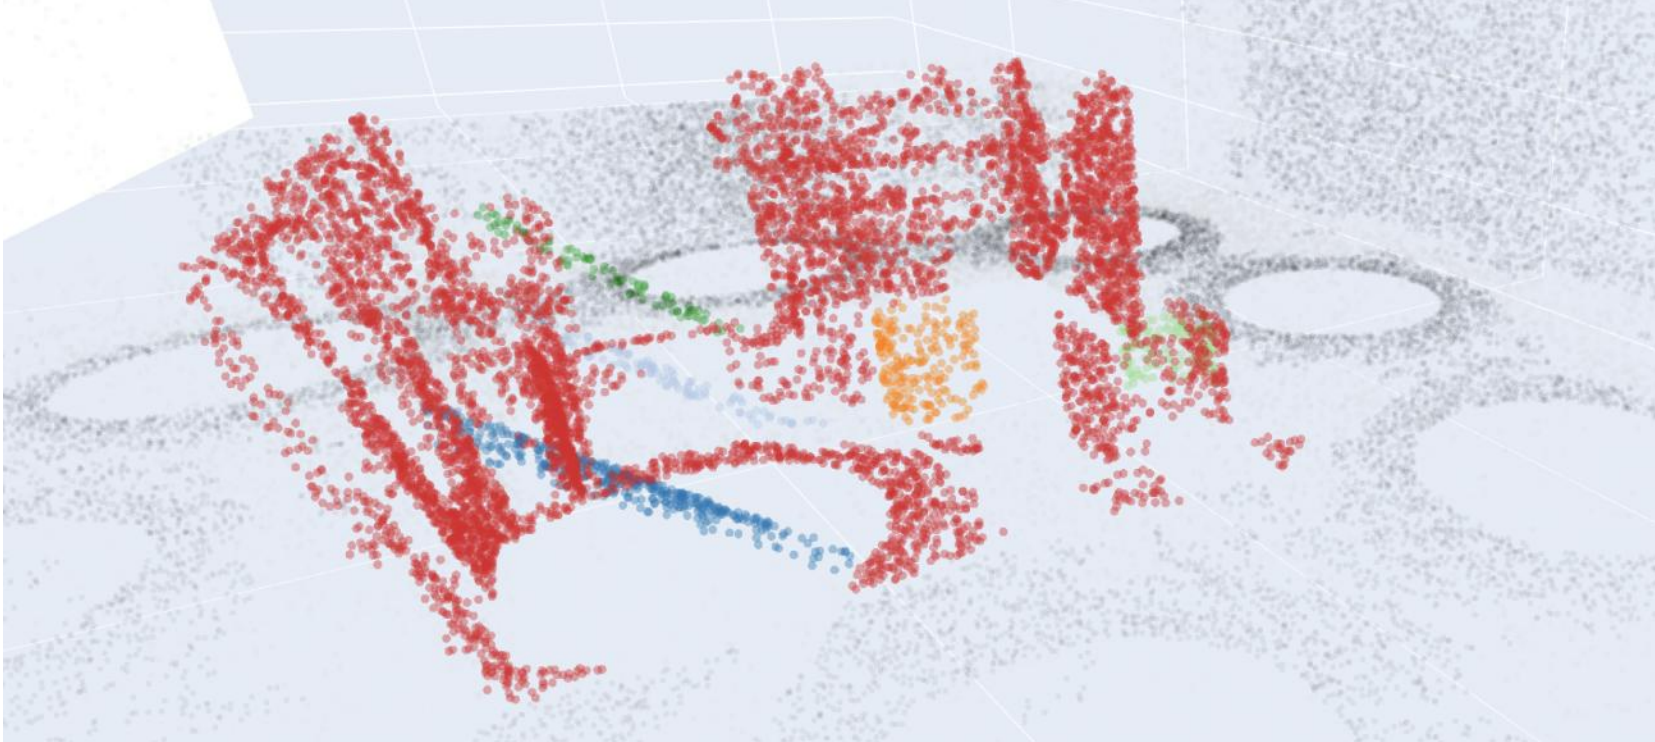
\includegraphics[width=\linewidth]{assets/shipyard.png}\par
\captiontext{Synthetic benchmark: 2 million points. Red: model-consistent; other colours: anomalies; grey: background. \textcopyright\ Naval Group \refb{6}.}
\vfill
\centering\resizebox{\linewidth}{!}{\begin{tikzpicture}[every node/.style={font=\fontsize{10}{11}\selectfont},
 b/.style={draw=inriablue,line width=.7pt,fill=white,rounded corners=1mm,
 minimum height=1.05cm,text width=2.65cm,align=center,inner sep=3pt}]
\node[b](a)at(0,0){HGP\\hierarchy};
\node[b](b)at(3.65,0){3D-model-guided\\tree selection};
\node[b](c)at(7.3,0){Anomaly\\instances};
\draw[-{Latex[length=2mm]},inriablue,line width=.8pt](a)--(b);
\draw[-{Latex[length=2mm]},inriablue,line width=.8pt](b)--(c);
\end{tikzpicture}
}\par
\vfill
\RaggedRight\textbf{Geometric priors select branches. No training required.}
\end{posterbox}
\gap
\begin{posterbox}[inriared]{5}{Perspective: geometry-guided 3D learning}{45.5cm}
\textbf{The same object, different sampling.}
\vspace{0.2cm}
\centering\resizebox{\linewidth}{!}{% Adapted from the defense at 3593fbf25434c4715b37537eae1287bf49239fa7; original blob 9cca660433532a16af3cf736cf9383184d3ba9e6.
                \begin{tikzpicture}[xscale=1.0, yscale=1.0]
                    \useasboundingbox (-0.45, -2.85) rectangle (13.35, 2.25);

                    \tikzset{pt/.style={circle, fill=inria-2024-bleu-canard, inner sep=0pt, minimum size=2.2pt}}
                    \tikzset{surf/.style={inria-rouge, line width=1.6pt, line join=round, line cap=round}}
                    \tikzset{carrosserie/.style={draw=gray!45, line width=0.7pt, fill=gray!8, line join=round}}
                    \tikzset{rayon/.style={gris_fonce_inria, line width=0.35pt, opacity=0.40}}
                    \tikzset{cadre/.style={draw=gray!30, line width=0.9pt, rounded corners=3pt}}

                    \newcommand{\voiture}{%
                        \draw[carrosserie]
                            (0.00,0.00) -- (0.00,0.42) -- (0.48,0.46) -- (0.92,0.98)
                            -- (2.00,0.98) -- (2.42,0.46) -- (3.00,0.42) -- (3.00,0.00) -- cycle;
                        \draw[gray!45, line width=0.7pt] (0.70,0.00) circle (0.20);
                        \draw[gray!45, line width=0.7pt] (2.30,0.00) circle (0.20);
                    }
                    \newcommand{\contour}{(0.00,0.42) (0.48,0.46) (0.92,0.98) (2.00,0.98) (2.42,0.46) (3.00,0.42)}

                    % ================== Panneau gauche : de près ==================
                    \begin{scope}[xshift=0.4cm, yshift=0.35cm]
                        \node[cadre, minimum width=5.0cm, minimum height=2.30cm] at (1.5,0.60) {};
                        \voiture
                        % Nappes de balayage tous les 0.108 : l'une longe le capot et le coffre
                        % (0.44), une autre le toit (0.98) ; chaque retour est à l'intersection
                        % d'une nappe et du contour (pas 0.108 le long d'une nappe).
                        \foreach \y in {0.224, 0.332, 0.440, 0.548, 0.656, 0.764, 0.872, 0.980, 1.088} {\draw[rayon] (-0.55,\y) -- (3.55,\y);}
                        \foreach \p in {(0.020,0.440),(0.128,0.440),(0.236,0.440),(0.344,0.440),(0.452,0.440),(0.555,0.548),(0.646,0.656),(0.738,0.764),(0.829,0.872),(0.980,0.980),(1.088,0.980),(1.196,0.980),(1.304,0.980),(1.412,0.980),(1.520,0.980),(1.628,0.980),(1.736,0.980),(1.844,0.980),(1.952,0.980),(2.087,0.872),(2.174,0.764),(2.261,0.656),(2.348,0.548),(2.450,0.440),(2.558,0.440),(2.666,0.440),(2.774,0.440),(2.882,0.440),(2.990,0.440)} {
                            \node[pt] at \p {};
                        }
                        \node[font=\fontsize{10}{11}\selectfont, text=gris_fonce_inria, anchor=north] at (1.5,-0.44) {\textbf{Near} object};
                    \end{scope}

                    % ================== Panneau droit : de loin ==================
                    \begin{scope}[xshift=6.9cm, yshift=0.35cm]
                        \node[cadre, minimum width=5.0cm, minimum height=2.30cm] at (1.5,0.60) {};
                        \voiture
                        % Nappes 2,5 fois plus espacées (0.27) et retours 3 fois plus espacés
                        % le long d'une nappe (0.34) : neuf retours sur trois nappes.
                        \foreach \y in {0.17, 0.44, 0.71, 0.98, 1.25} {\draw[rayon] (-0.55,\y) -- (3.55,\y);}
                        \foreach \p in {(0.080,0.440),(0.420,0.440),(0.692,0.710),(1.100,0.980),(1.440,0.980),(1.780,0.980),(2.218,0.710),(2.580,0.440),(2.920,0.440)} {
                            \node[pt] at \p {};
                        }
                        \node[font=\fontsize{10}{11}\selectfont, text=gris_fonce_inria, anchor=north] at (1.5,-0.44) {\textbf{Far} object};
                    \end{scope}

                    % ================== Flèches ==================
                    \draw[-{Latex[length=2.8mm]}, line width=1.6pt, color=gray!45] (1.90,-0.95) -- (1.90,-1.28);
                    \draw[-{Latex[length=2.8mm]}, line width=1.6pt, color=gray!45] (8.40,-0.95) -- (8.40,-1.28);

                    % ================== Surfaces reconstruites ==================
                    % à gauche : fine ; à droite : grossière, mais même cible
                    \begin{scope}[xshift=0.4cm, yshift=-2.40cm]
                        \draw[gray!45, line width=0.7pt, densely dotted] plot coordinates {\contour};
                        \draw[surf] plot coordinates {\contour};
                    \end{scope}
                    \begin{scope}[xshift=6.9cm, yshift=-2.40cm]
                        \draw[gray!45, line width=0.7pt, densely dotted] plot coordinates {\contour};
                        % La surface interpole les neuf retours observés : ses sommets sont
                        % sur le contour gris, les cordes coupent les angles. Grossière, mais
                        % c'est bien le même objet, c'est tout le propos de la planche.
                        \draw[surf] plot coordinates {(0.080,0.440) (0.420,0.440) (0.692,0.710) (1.100,0.980) (1.440,0.980) (1.780,0.980) (2.218,0.710) (2.580,0.440) (2.920,0.440)};
                    \end{scope}

                    % Both comparison signs share the midpoint between the two panels.
\def\comparisonx{5.15}
\node[font=\fontsize{18}{20}\selectfont\bfseries, text=inriablue] at (\comparisonx,0.95) {$\ne$};
\node[font=\fontsize{18}{20}\selectfont\bfseries, text=inria-rouge] at (\comparisonx,-1.86) {$\approx$};

                    \node[font=\fontsize{8}{9}\selectfont, text=inria-2024-bleu-canard, anchor=east, align=right] at (12.45,0.95)
                        {\textbf{Sampling}\\depends on\\sensor and range};
                    \node[font=\fontsize{8}{9}\selectfont, text=inria-rouge, anchor=east, align=right] at (12.45,-1.90)
                        {\textbf{Geometry}\\may vary less\\(hypothesis)};
                \end{tikzpicture}
}\par
\captiontext{Range, scan pattern and occlusion change the point cloud. Surface geometry may be more stable.}
\vfill
\RaggedRight\textbf{Polyhedra as tokens; hierarchy as multiscale context.}
\vspace{0.25cm}
\centering\resizebox{0.78\linewidth}{!}{% Adapted from the defense at 3593fbf25434c4715b37537eae1287bf49239fa7; original blob a0d8fff49a7ccd75cf59e7a16094ddb209e4cdde.
                    % Hierarchie de K-polyedres proposee comme unite de calcul a la place du point.
                    % Les six pieces des feuilles sont les six secteurs d'un meme polygone maitre
                    % irregulier (decoupe en eventail autour d'un point interieur O). Elles sont
                    % dessinees partout a la meme echelle et dans la meme orientation : le polyedre
                    % d'un noeud interne est donc litteralement le recollement de ceux de ses deux
                    % enfants, soude le long de la face tracee en rouge epais. L'ordonnee est le
                    % rayon physique r ; le point rouge d'un noeud est place en O, au coeur du polyedre.
                    \begin{tikzpicture}[xscale=1.0, yscale=1.0]
                    \useasboundingbox (-1.70, -0.40) rectangle (10.303, 7.541);

                    \tikzset{arbre/.style={gris_fonce_inria!75, line width=0.9pt}}
                    \tikzset{bord/.style={draw=inria-2024-bleu-canard, line width=1.05pt, line join=round}}
                    \tikzset{couture/.style={draw=inria-2024-bleu-canard!70, line width=0.4pt}}
                    \tikzset{soudure/.style={draw=inria-rouge, line width=1.7pt}}

                    % ==== axe des rayons ====
                    \draw[-{Latex[length=2.4mm]}, gris_fonce_inria, line width=0.8pt] (-1.00,-0.25) -- (-1.00,7.271);
                    \node[font=\fontsize{8}{9}\selectfont, text=gris_fonce_inria, anchor=south] at (-1.00,7.341) {$r$};
                    \draw[gris_fonce_inria, line width=0.6pt] (-1.00,0.6) -- (-0.84,0.6);
                    \draw[gris_fonce_inria, line width=0.6pt] (-1.00,1.2) -- (-0.84,1.2);
                    \draw[gris_fonce_inria, line width=0.6pt] (-1.00,2.4) -- (-0.84,2.4);
                    \draw[gris_fonce_inria, line width=0.6pt] (-1.00,3.6) -- (-0.84,3.6);
                    \draw[gris_fonce_inria, line width=0.6pt] (-1.00,4.8) -- (-0.84,4.8);
                    \draw[gris_fonce_inria, line width=0.6pt] (-1.00,6) -- (-0.84,6);
                    \node[rotate=90, font=\fontsize{8}{9}\selectfont, text=gris_fonce_inria, anchor=south] at (-1.50,2.88) {merging radius};

                    % ==== arbre (passe derriere les polyedres) ====
                    \draw[arbre] (5.9,0.528) -- (5.9,1.92);
                    \draw[arbre] (4.1,0.912) -- (4.1,1.92);
                    \draw[arbre] (5.9,1.92) -- (4.1,1.92);
                    \draw[arbre] (0.5,0.312) -- (0.5,2.4);
                    \draw[arbre] (2.3,0.744) -- (2.3,2.4);
                    \draw[arbre] (0.5,2.4) -- (2.3,2.4);
                    \draw[arbre] (7.7,1.056) -- (7.7,2.76);
                    \draw[arbre] (9.5,0.624) -- (9.5,2.76);
                    \draw[arbre] (7.7,2.76) -- (9.5,2.76);
                    \draw[arbre] (5,1.92) -- (5,4.2);
                    \draw[arbre] (1.4,2.4) -- (1.4,4.2);
                    \draw[arbre] (5,4.2) -- (1.4,4.2);
                    \draw[arbre] (3.2,4.2) -- (3.2,6.24);
                    \draw[arbre] (8.6,2.76) -- (8.6,6.24);
                    \draw[arbre] (3.2,6.24) -- (8.6,6.24);

                    % ==== polyedres : un par noeud, a sa hauteur ====
                    % noeud p1
                    \fill[inria-2024-bleu-canard!12] (5.397,0.321) -- (6.403,0.445) -- (6.103,0.735) -- cycle;
                    \draw[bord] (5.397,0.321) -- (6.403,0.445) -- (6.103,0.735) -- cycle;
                    % noeud p2
                    \fill[inria-2024-bleu-canard!58] (3.902,0.582) -- (4.608,0.996) -- (4.103,1.242) -- (3.592,1.048) -- cycle;
                    \draw[bord] (3.902,0.582) -- (4.608,0.996) -- (4.103,1.242) -- (3.592,1.048) -- cycle;
                    % noeud p3
                    \fill[inria-2024-bleu-canard!30] (0.936,0.274) -- (0.626,0.74) -- (0.064,0.627) -- (0.131,0.294) -- (0.14,-0.116) -- cycle;
                    \draw[bord] (0.936,0.274) -- (0.626,0.74) -- (0.064,0.627) -- (0.131,0.294) -- (0.14,-0.116) -- cycle;
                    % noeud p4
                    \fill[inria-2024-bleu-canard!78] (2.698,1.095) -- (1.902,0.704) -- (2.43,0.393) -- cycle;
                    \draw[bord] (2.698,1.095) -- (1.902,0.704) -- (2.43,0.393) -- cycle;
                    % noeud p5
                    \fill[inria-2024-bleu-canard!42] (7.547,1.407) -- (7.279,0.705) -- (7.745,0.89) -- (8.121,0.928) -- cycle;
                    \draw[bord] (7.547,1.407) -- (7.279,0.705) -- (7.745,0.89) -- (8.121,0.928) -- cycle;
                    % noeud p6
                    \fill[inria-2024-bleu-canard!95] (8.997,0.801) -- (9.57,0.322) -- (9.897,0.507) -- (9.843,0.749) -- (10.003,0.926) -- cycle;
                    \draw[bord] (8.997,0.801) -- (9.57,0.322) -- (9.897,0.507) -- (9.843,0.749) -- (10.003,0.926) -- cycle;
                    % noeud A
                    \fill[inria-2024-bleu-canard!12] (4.652,1.59) -- (5.659,1.714) -- (5.358,2.004) -- cycle;
                    \fill[inria-2024-bleu-canard!58] (4.652,1.59) -- (5.358,2.004) -- (4.852,2.25) -- (4.341,2.056) -- cycle;
                    \draw[bord] (4.652,1.59) -- (5.659,1.714) -- (5.358,2.004) -- (4.852,2.25) -- (4.341,2.056) -- cycle;
                    \draw[soudure] (4.652,1.59) -- (5.358,2.004);
                    % noeud B
                    \fill[inria-2024-bleu-canard!30] (1.836,2.518) -- (1.526,2.983) -- (0.964,2.87) -- (1.031,2.537) -- (1.04,2.127) -- cycle;
                    \fill[inria-2024-bleu-canard!78] (1.836,2.518) -- (1.04,2.127) -- (1.568,1.817) -- cycle;
                    \draw[bord] (1.836,2.518) -- (1.526,2.983) -- (0.964,2.87) -- (1.031,2.537) -- (1.04,2.127) -- (1.568,1.817) -- cycle;
                    \draw[soudure] (1.836,2.518) -- (1.04,2.127);
                    % noeud C
                    \fill[inria-2024-bleu-canard!42] (8.231,3.048) -- (7.962,2.347) -- (8.428,2.532) -- (8.805,2.57) -- cycle;
                    \fill[inria-2024-bleu-canard!95] (8.231,3.048) -- (8.805,2.57) -- (9.131,2.754) -- (9.077,2.997) -- (9.238,3.173) -- cycle;
                    \draw[bord] (8.231,3.048) -- (7.962,2.347) -- (8.428,2.532) -- (8.805,2.57) -- (9.131,2.754) -- (9.077,2.997) -- (9.238,3.173) -- cycle;
                    \draw[soudure] (8.231,3.048) -- (8.805,2.57);
                    % noeud D
                    \fill[inria-2024-bleu-canard!12] (3.133,4.22) -- (4.14,4.344) -- (3.839,4.635) -- cycle;
                    \fill[inria-2024-bleu-canard!58] (3.133,4.22) -- (3.839,4.635) -- (3.334,4.881) -- (2.823,4.686) -- cycle;
                    \fill[inria-2024-bleu-canard!30] (3.133,4.22) -- (2.823,4.686) -- (2.26,4.573) -- (2.327,4.24) -- (2.337,3.83) -- cycle;
                    \fill[inria-2024-bleu-canard!78] (3.133,4.22) -- (2.337,3.83) -- (2.865,3.519) -- cycle;
                    \draw[couture] (3.133,4.22) -- (3.839,4.635);
                    \draw[couture] (3.133,4.22) -- (2.337,3.83);
                    \draw[bord] (3.133,4.22) -- (4.14,4.344) -- (3.839,4.635) -- (3.334,4.881) -- (2.823,4.686) -- (2.26,4.573) -- (2.327,4.24) -- (2.337,3.83) -- (2.865,3.519) -- cycle;
                    \draw[soudure] (3.133,4.22) -- (2.823,4.686);
                    % noeud R
                    \fill[inria-2024-bleu-canard!12] (5.833,6.26) -- (6.84,6.384) -- (6.539,6.675) -- cycle;
                    \fill[inria-2024-bleu-canard!58] (5.833,6.26) -- (6.539,6.675) -- (6.034,6.921) -- (5.523,6.726) -- cycle;
                    \fill[inria-2024-bleu-canard!30] (5.833,6.26) -- (5.523,6.726) -- (4.96,6.613) -- (5.027,6.28) -- (5.037,5.87) -- cycle;
                    \fill[inria-2024-bleu-canard!78] (5.833,6.26) -- (5.037,5.87) -- (5.565,5.559) -- cycle;
                    \fill[inria-2024-bleu-canard!42] (5.833,6.26) -- (5.565,5.559) -- (6.031,5.744) -- (6.407,5.781) -- cycle;
                    \fill[inria-2024-bleu-canard!95] (5.833,6.26) -- (6.407,5.781) -- (6.734,5.966) -- (6.679,6.208) -- (6.84,6.384) -- cycle;
                    \draw[couture] (5.833,6.26) -- (6.539,6.675);
                    \draw[couture] (5.833,6.26) -- (5.523,6.726);
                    \draw[couture] (5.833,6.26) -- (5.037,5.87);
                    \draw[couture] (5.833,6.26) -- (6.407,5.781);
                    \draw[bord] (6.84,6.384) -- (6.539,6.675) -- (6.034,6.921) -- (5.523,6.726) -- (4.96,6.613) -- (5.027,6.28) -- (5.037,5.87) -- (5.565,5.559) -- (6.031,5.744) -- (6.407,5.781) -- (6.734,5.966) -- (6.679,6.208) -- (6.84,6.384) -- cycle;
                    \draw[soudure] (5.833,6.26) -- (5.565,5.559);
                    \draw[soudure] (5.833,6.26) -- (6.84,6.384);

                    % ==== noeuds : le point de fusion, au centre du polyedre ====
                    \fill[inria-rouge] (5.9,0.528) circle (2.0pt);
                    \fill[inria-rouge] (4.1,0.912) circle (2.0pt);
                    \fill[inria-rouge] (0.5,0.312) circle (2.0pt);
                    \fill[inria-rouge] (2.3,0.744) circle (2.0pt);
                    \fill[inria-rouge] (7.7,1.056) circle (2.0pt);
                    \fill[inria-rouge] (9.5,0.624) circle (2.0pt);
                    \fill[inria-rouge] (5,1.92) circle (2.6pt);
                    \fill[inria-rouge] (1.4,2.4) circle (2.6pt);
                    \fill[inria-rouge] (8.6,2.76) circle (2.6pt);
                    \fill[inria-rouge] (3.2,4.2) circle (2.6pt);
                    \fill[inria-rouge] (5.9,6.24) circle (3.0pt);

                    \end{tikzpicture}
}\par
\captiontext{Each parent joins its children along shared faces (red). Schematic geometry and merging radii.}
\vfill
\centering\resizebox{\linewidth}{!}{\begin{tikzpicture}[box/.style={draw=inriared,fill=white,rounded corners=2pt,line width=.8pt,text width=3.1cm,minimum height=1.12cm,align=center,font=\fontsize{11}{12}\selectfont},>={Latex[length=2mm]}]
\node[box](a)at(0,0){Polyhedral\\components};
\node[box](b)at(4.4,0){Vector tokens\\$z_v$};
\node[box](c)at(8.8,0){Hierarchy-guided\\3D backbone};
\draw[->,inriared,line width=.9pt](a)--(b);
\draw[->,inriared,line width=.9pt](b)--(c);
\end{tikzpicture}
}\par
\vspace{0.4cm}
\RaggedRight\smalltext{\textcolor{inriared}{\textbf{Research hypothesis:}} guide a 3D foundation model with geometric tokens and their merging scales. Learning gains remain to be tested.}
\end{posterbox}
\gap
\begin{posterbox}{6}{Inria Startup Studio: Percolia}{6.0cm}
\vfill
\begin{minipage}[c]{0.14\linewidth}\centering

\includegraphics[width=4.2cm]{assets/percolia-p.pdf}
\end{minipage}\hfill
\begin{minipage}[c]{0.61\linewidth}
\textbf{Louis \textsc{Hauseux} \& Alban \textsc{Hauseux}}\par
\smalltext{Entering \textbf{Inria Startup Studio}.}
\vspace{0.2cm}
\smalltext{Geometry-aware tools for 3D perception.}
\end{minipage}\hfill
\begin{minipage}[c]{0.20\linewidth}\centering
{\hypersetup{urlcolor=black}\qrcode[height=4.3cm,hyperlink=false]{\PercoliaLinkedIn}}\par
\vspace{0.18cm}{\fontsize{23}{26}\selectfont\href{\PercoliaLinkedIn}{LinkedIn}\par}
\end{minipage}
\vfill
\end{posterbox}
\end{column}
\end{columns}
\vspace{0.65cm}
\begin{posterbox}{7}{References}{5.8cm}
\begingroup
\fontsize{22}{25}\selectfont\color{inriagrayblue}
\setlength{\columnsep}{1.4cm}\setlength{\parskip}{0.13cm}
\vspace{-0.15cm}
\begin{multicols}{2}\RaggedRight
\refb{1} J. A. Hartigan. \emph{Consistency of single linkage for high-density clusters}. JASA, 76:388--394, 1981.\par
\refb{2} G. Biau and L. Devroye. \emph{Lectures on the Nearest Neighbor Method}. Springer, 2015.\par
\refb{3} R. J. G. B. Campello, D. Moulavi and J. Sander. \emph{Density-Based Clustering Based on Hierarchical Density Estimates}. PAKDD, pp.~160--172, 2013.\par
\columnbreak
\myref{4} L. Hauseux, K. Avrachenkov and J. Zerubia. {\hypersetup{urlcolor=inriared}\href{https://doi.org/10.1007/s41109-025-00756-1}{\emph{Generalization of single-linkage with higher-order interactions}}}. Applied Network Science, 11, article 9, 2026.\par
\myref{5} L. Hauseux, K. Avrachenkov and J. Zerubia. {\hypersetup{urlcolor=inriared}\href{https://doi.org/10.23919/EUSIPCO63174.2024.10715271}{\emph{Benefits of hypergraphs for density-based clustering}}}. EUSIPCO, pp.~2302--2306, 2024.\par
\refb{6} AYANA team. \href{https://radar.inria.fr/report/2025/ayana/index.html\#AYANA-RA-2025_label_NavalResult}{\emph{3D LiDAR Instance Segmentation with Geometric Priors: The HGP-Clusterer}}. Inria Annual Report 2025, \S7.7.\par
\end{multicols}
\endgroup

\end{posterbox}
\end{frame}
\end{document}
